% ======================================================================
% ======================================================================
% ======================================================================
%
% UNOFFICIAL style for Posters at RU-DI
% Radboud University, Donders Institute,
% Nijmengen, Netherlands
%
%     Author: Riccardo Metere <r.metere@donders.ru.nl>
%       Date: Jun 2018
%  Copyright: 2018 (C) Riccardo Metere
%    License: LaTeX Project Public License (LPPL) 
%
% Instructions:
% - Look for `%FIXME` for finding items requiring author's attention
% - Read the comments and if something is unclear please drop me a note
%
% TODO:
% - Improve on the citation handling
% - Improve on the figure reference handling
% ======================================================================
% ======================================================================
% ======================================================================


% ======================================================================
% : initial configuration
\documentclass[portrait,a0paper]{rudi-poster}  % FIXME (landscape|portrait)

%%% Customisation
% Determine whether it is local compilation or overleaf compilation
\makeatletter
\begingroup\endlinechar=-1\relax
       \everyeof{\noexpand}%
       \edef\x{\endgroup\def\noexpand\homepath{%
         \@@input|"kpsewhich --var-value=HOME" }}\x
\makeatother
\def\overleafhome{/tmp}% change as appropriate

% Include algorithm.
\usepackage{cleveref}
\usepackage[ruled,linesnumbered]{algorithm2e}

% Global change of algorithm input output naming.
\SetKwInput{KwData}{Input}
\SetKwInput{KwResult}{Output}

% Color words red.
\usepackage{xcolor}

% Include audio to turn into poster
\usepackage{media9}

% Allow to use cmdrule to draw horizontal line in table.
\usepackage{booktabs}
\usepackage{multirow}

% Compact lists
%\usepackage{enumitem}
%%% End customisation


% : additional packages
\usepackage[T1]{fontenc}  % Standard package for selecting font encodings
\usepackage[utf8x]{inputenc}  % Accept different input encodings
\usepackage{mathtools}  % Mathematical tools to use with amsmath
% \usepackage[english]{babel}  % Multilingual support for Plain TeX or LaTeX
\usepackage{amsmath}  % AMS mathematical facilities for LaTeX
\usepackage{amsfonts}  % TeX fonts from the American Mathematical Society

\usepackage{wasysym}  % LaTeX support file to use the WASY2 fonts
\usepackage{bbm}  % "Blackboard-style" cm fonts
\usepackage{array}  % Extending the array and tabular environments
\usepackage{verbatim}  % Reimplementation of and extensions to LaTeX verbatim
\usepackage{float}  % Improved interface for floating objects
\usepackage[inline]{enumitem}  % Control layout of itemize, enumerate, description
\usepackage{qrcode}  % Generate QR codes in LaTeX
\usepackage{lipsum}

%\usepackage{enumitem}
\usepackage{cleveref}

%\usepackage{amssymb}  % Additional symbols from American Mathematical Society
% ======================================================================
% : set-up document information  % FIXME
\title{Leveraging brain-adaptation principles to increase radiation\\
resistance of neuromorphic space hardware}
%\includemedia[
%  addresource=audio/output/1_4_short_text.mp3,
%  transparent,
%  flashvars={
%    source=audio/output/1_4_short_text.mp3
%   &autoPlay=true
%  },
%]{\includegraphics[height=0.8em]{audio/speaker.png}}{APlayer.swf}}
% \title{RU-DI Poster Template RU-DI Poster Template RU-DI Poster Template RU-DI Poster Template RU-DI Poster Template RU-DI Poster Template}  % STRESS-TEST
%\author{Akke Toeter, J.H.P. Kwisthout, D.M. Stam, A. Menicucci}
\author{Akke Toeter}
%\author{J.H.P. Kwisthout}
%\author{D.M. Stam}
%\author{A. Menicucci}
\date{2022-07-28}



\newcommand{\Contact}{e-mail: \mailto{akke.toeter@radboud.student.nl}}
\newcommand{\Authors}{
	\hspace{-1ex}
    \begin{itemize*}[label=]
        %\item Custom text
    	\item \theauthor\textsuperscript{1,2} %,
        \item J.H.P. Kwisthout\textsuperscript{1} %,
        \item D.M.Stam\textsuperscript{2} %,
        \item A. Menicucci\textsuperscript{2} %,
        %\item \theauthor\textsuperscript{1} %,
        %\item \theauthor\textsuperscript{2} %,
        %\item \theauthor\textsuperscript{2} %,
% 	    \item \theauthor\textsuperscript{1}  % STRESS-TEST
% 	    \item \theauthor\textsuperscript{1}  % STRESS-TEST
% 	    \item \theauthor\textsuperscript{1}  % STRESS-TEST
% 	    \item \theauthor\textsuperscript{1}  % STRESS-TEST
    \end{itemize*}}
\newcommand{\Affiliations}{
%   \hspace{0.1ex}
  \begin{enumerate*}[label=\textbf{\arabic*} ]
    \item \RUDI, Nijmegen, Netherlands
    \item \DELFT, Delft, Netherlands
%     \item \RUDI  % STRESS-TEST
%     \item \RUDI  % STRESS-TEST
%     \item \RUDI  % STRESS-TEST
%     \item \RUDI  % STRESS-TEST
  \end{enumerate*}}
  
\newcommand{\ExtraLogos}{%
	\qrcode[height=\rudisizeextralogo]{https://github.com/a-t-0/networkx-to-lava-nc/}}

\newcommand{\EventName}{ICONS}
\newcommand{\EventLocation}{Knoxville, Tennessee (USA)>}
\newcommand{\PresentedAt}{Presented at the \EventName{} in \EventLocation{} on \theeventdate}

\newcommand{\References}{
    \textbf{References}%\par
    %\begin{enumerate*}[label={[}\textbf{\arabic*}{]}]
    \begin{enumerate}
    \itemsep-1em 
\item  M. Ben-Menachem and I. Gavious, 2007, Accounting Software Assets:A Valuation Model for Software,  Ben-Gurion University.\\ % Business model
\item Royal Dutch Airlines KLM Annual Report 2019.\\ % anual report
\item S. Shahrivar et al., 2018, A business model for commercial open source software: A systematic literature review, Tarbiat Modares University.\\ % COSS 
\item G. Schryen and R. Kadura, 2009, Open Source vs. Closed Source Software: Towards Measuring Security. % Security can add safety
\end{enumerate}}
\newcommand{\Acknowledgments}{
	\textbf{Acknowledgments}:
    \begin{itemize*}[label=]
    	\item Dr. W.F.G. Haselager for suggesting open source software as topic for a research brief.
    \end{itemize*}}
% \newcommand{\Funding}{
% 	\textbf{Funded by}:
%     \begin{itemize*}[label=]
%     	\item T.b.d.
%     \end{itemize*}}
\newcommand{\Keywords}{
	Magnetic Resonance Imaging,
    MRI,
    Nuclear Magnetic Resonance,
    NMR}

% ======================================================================
% fill in PDF metadata
\hypersetup{% hyperref setup for PDFs
  pdftitle={\theauthor{}~-~\thetitle{}~-~(\EventName{},~\theyear{})},
  pdfcreationdate={\thedate{}},
  pdfauthor={\theauthor{}},
  pdfkeywords={\Keywords{}},
  pdflang={\languagename},
}%

% ======================================================================
% :: adjust block sizes  % FIXME
% : block sizes
% \setlength{\rudisizeblockheader}{0.077\paperheight}
% \setlength{\rudisizeblockintro}{0.087\paperheight}
% \setlength{\rudisizeblockmethods}{0.099\paperheight}
% \setlength{\rudisizeblockdiscussion}{0.130\paperheight}
% % set length to vertical fill space of results block
% \setlength{\rudisizeblockresults}{\paperheight - \rudisizeblockheader - \rudisizeblockintro - \rudisizeblockmethods - \rudisizeblockdiscussion - 0\rudisizeblocktitleheight - 4\parskip - 2\rudisizemargin - 8\rudisizevpadding - 10\rudisizeborder + 6\uum - 0\uum}
% % set length of Addendum block equal to Discussion block
% \setlength{\rudisizeblockaddendum}{\rudisizeblockdiscussion}


% ======================================================================
%% Document
\begin{document}

% Compact lists
% \renewcommand{\@listI}{%
% \leftmargin=25pt
% \rightmargin=0pt
% \labelsep=0pt
% \labelwidth=20pt
% \itemindent=0pt
% \listparindent=0pt
% \topsep=0pt plus 2pt minus 4pt
% \partopsep=0pt plus 1pt minus 1pt
% \parsep=0pt plus 1pt
% \itemsep=\parsep}


% ======================================================================
\rudiposterheader{\thetitle}{\Authors}{\Affiliations}
\rudipostersidenote{\PresentedAt}
\rudiposterfooter{\Contact}{\ExtraLogos}

% ======================================================================
\vspace{-2.4em}
\begin{rudiblockintro}
    \begin{multicols}{3}
        %% The abstract is a short summary of the work to be presented in the
%% article.
        
        \ifx\homepath\overleafhome
            % Overleaf compilation.
            %\begin{abstract}
  %Energy efficient applications of artificial intelligence (AI) may be able to increase space robot autonomy. 
  This research sets out to test whether principles of brain adaptation can be leveraged to increase the radiation resistance of neuromorphic space hardware. Neuromorphic architectures provide energy efficient platforms for AI applications in space. Structural similarities between neuromorphic architectures and the brain may allow them to benefit from brain-inspired design on the topic of damage recovery. Space environments can provide challenging conditions with significant radiation exposure, that may damage neuromorphic space hardware. To explore approaches to mitigate such damages, a simulated radiation test with- and without a brain inspired implementation adaptation is investigated. These adaptations are applied to a spiking neural network (SNN) implementation of a distributed minimum dominating set approximation algorithm by Alipour et al. The experiment is performed using Intel's Lava 0.3.0 Framework. With radiation induced neuron death probabilities of 25\%, adaptation increased SNN robustness, compared to no adaptation. At lower neuron death probabilities, no difference is observed.
 % Include audio file.
%\end{abstract}
        \else
            % Local compilation
            %\begin{abstract}
  %Energy efficient applications of artificial intelligence (AI) may be able to increase space robot autonomy. 
  This research sets out to test whether principles of brain adaptation can be leveraged to increase the radiation resistance of neuromorphic space hardware. Neuromorphic architectures provide energy efficient platforms for AI applications in space. Structural similarities between neuromorphic architectures and the brain may allow them to benefit from brain-inspired design on the topic of damage recovery. Space environments can provide challenging conditions with significant radiation exposure, that may damage neuromorphic space hardware. To explore approaches to mitigate such damages, a simulated radiation test with- and without a brain inspired implementation adaptation is investigated. These adaptations are applied to a spiking neural network (SNN) implementation of a distributed minimum dominating set approximation algorithm by Alipour et al. The experiment is performed using Intel's Lava 0.3.0 Framework. With radiation induced neuron death probabilities of 25\%, adaptation increased SNN robustness, compared to no adaptation. At lower neuron death probabilities, no difference is observed.
 % Include audio file.
%\end{abstract}
        \fi
    \end{multicols}
\end{rudiblockintro}



% ======================================================================

%\begin{rudiblockmethods}
%\end{rudiblockmethods}

% ======================================================================

\begin{rudiblockiintroduction}
    \begin{multicols}{3}
        \ifx\homepath\overleafhome
            % Overleaf compilation.
            %\section{Methodology}\label{sec:methodology}
\colchunk[1]{%
        %EDUCATION\\*
        %\\*[.5\baselineskip]
        %\\*
%\titlespacing*{\subsection}{1pt}{1.1\baselineskip}{\baselineskip}        
\vspace{-40em}
\section{Select Distributed Algorithm}\label{subsec:algorithm}
The Minimum Dominating Set Approximation algorithm as presented by Alipour et al., is specified as:
%Within the graph algorithms, some SNN algorithms may be naturally more robust than others. For example, SNN algorithms that calculate the shortest path within graphs may automatically re-route if radiation imposed neuron-death occurs. However, since this research aims at determining the effectivity of brain adaptation mechanisms, a stricter test is found in algorithms that can fail to produce meaningful output if a single neuronal or synaptic property is changed. Therefore, 
%\begin{algorithm}%[h]%[1]
    %\caption{Distributed Algorithm for computing a total dominating set in a graph with given integer $m\geq 0$.}\label{alg:alipour}

%\KwData*
\textbf{Input:}\textit{Connected, planar, triangle-free graph of size $n$.}\\
%\KwResult*{\textit{Set of nodes that form a minimum total dominating set.}}
\textbf{Output:}\textit{Set of nodes that form a minimum total dominating set.}\\
%\setlist{nolistsep}
\vspace{-1.5em}
\begin{enumerate}[noitemsep]
\itemsep-1.5em
\item \textit{In the first round, each node $v_i$ chooses a random number $0<r_i<1$, computes degree $d_i$ and computes its weight $w_i=d_i+r_i$ and sends $w_i$ to its adjacent neighbours.}\\
\item \textit{In the second round, each node $v$ marks a neighbour vertex $v_i$ whose weight $w_i$ is maximum among all the other neighbours of $v$.}\\
\For{$m$ rounds}{
    \begin{enumerate}[noitemsep]
        \itemsep-1.5em
    \item \textit{Let $x_i$ be the number of times that a vertex is marked by its neighbour vertices, let $w_i=x_i+r_i$}\\
    \item \textit{Unmark the marked vertices.}\\
    \item \textit{Each vertex marks the vertex with maximum $w_i$ among its neighbour vertices.}\\
    \end{enumerate}
}
\vspace{1.5em}
\item \textit{The marked vertices are considered as the vertices in our total dominating set for $G$.}
\end{enumerate}
%\end{algorithm}

\section{Convert Algorithm to Spiking Neural Network(SNN)}\label{subsec:algo_to_snn}
%\vspace{-1.5em}
Next, an SNN implementation of this algorithm is generated using Leaky-Integrate-and-Fire (LIF) neurons. This implementation takes as input connected, triangle-free, planar graphs (E.g. Fig 1.). Then it converts these graphs into the specification of an SNN that is encoded in a new graph (E.g. Fig 2.). These graphs can then be simulated using the Lava backend by Loihi, or a custom Networkx SSN simulator backend.

\section{Apply Adaptation Mechanism to SNN}\label{subsec:adaptation}
The SNN is enhanced with redundant neurons, that are by default inhibited by their original neuron (Fig. 3). If the original neuron dies, the redundant neuron automatically takes over. 


\section{Simulate Radiation on SNN}\label{subsec:}
Space radiation damage is simulated in the form of random neuron deaths. Redundant neurons can die too (see red neuron pairs in Fig 4).. \vspace{-7em}
\section{Compare SNN Performance With-/out Adaptation}\label{subsec:}
%Algorithm performance during simulated radiation exposure, is compared with/without the adaptation mechanism.\\
SNN performance during simulated radiation exposure is compared with/without adaptation.\\
%\\*[.5\baselineskip]
\\*
%\begin{figure}[]
%    \centering
%    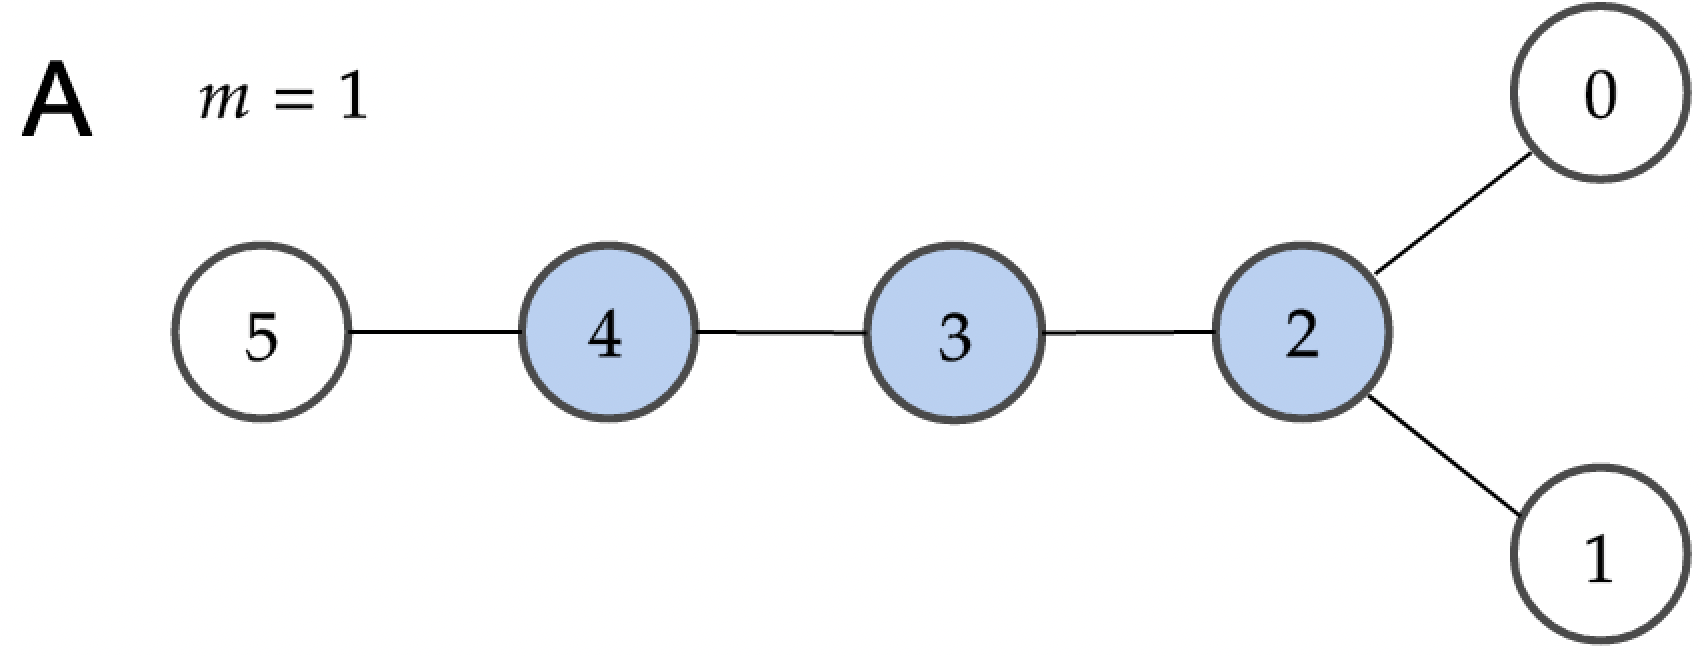
\includegraphics[width=8cm]{latex/Images/input_graph_G_6_0_alternative1.png}
%    \caption{Example input graph. For $m=1$ the algorithm still selects 3 nodes as it is an approximation of the MDS.}
%    \label{fig:input_graph}
%\end{figure}
%\hspace{-3em}
\vspace{-45em}
\begin{rudifig}{0.49\hsize}{Fig. 1: Input Graph}
%\begin{rudifig}{Fig. 1: Input Graph}
    \hspace{-1.5em}
    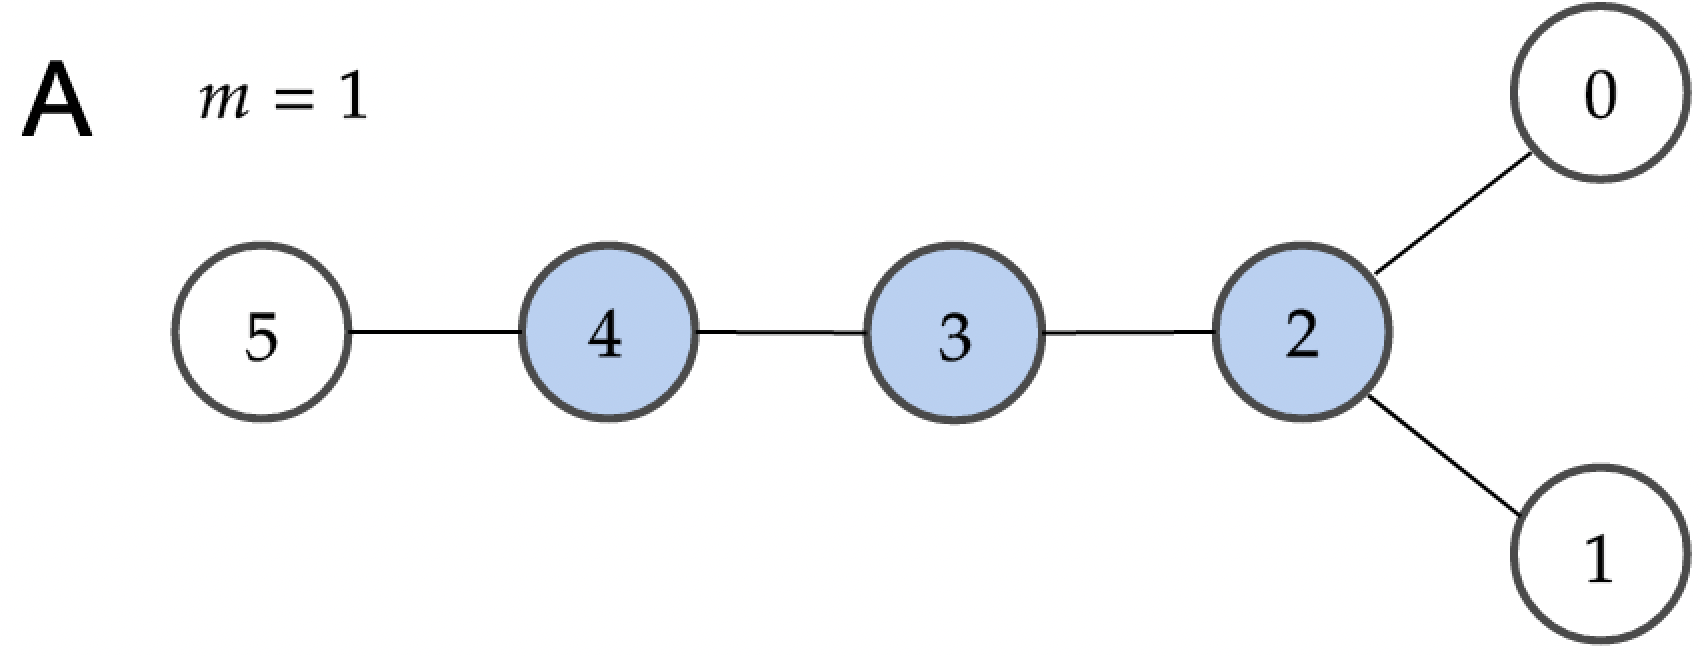
\includegraphics[width=1.1\linewidth]{latex/Images/input_graph_G_6_0_alternative1.png}
    %\caption{Example input graph. For $m=1$ the algorithm still selects 3 nodes as it is an approximation of the MDS.}
    \label{fig:input_graph}
\end{rudifig}
% Non poster image:
%\begin{figure}[H]
%    \centering
%    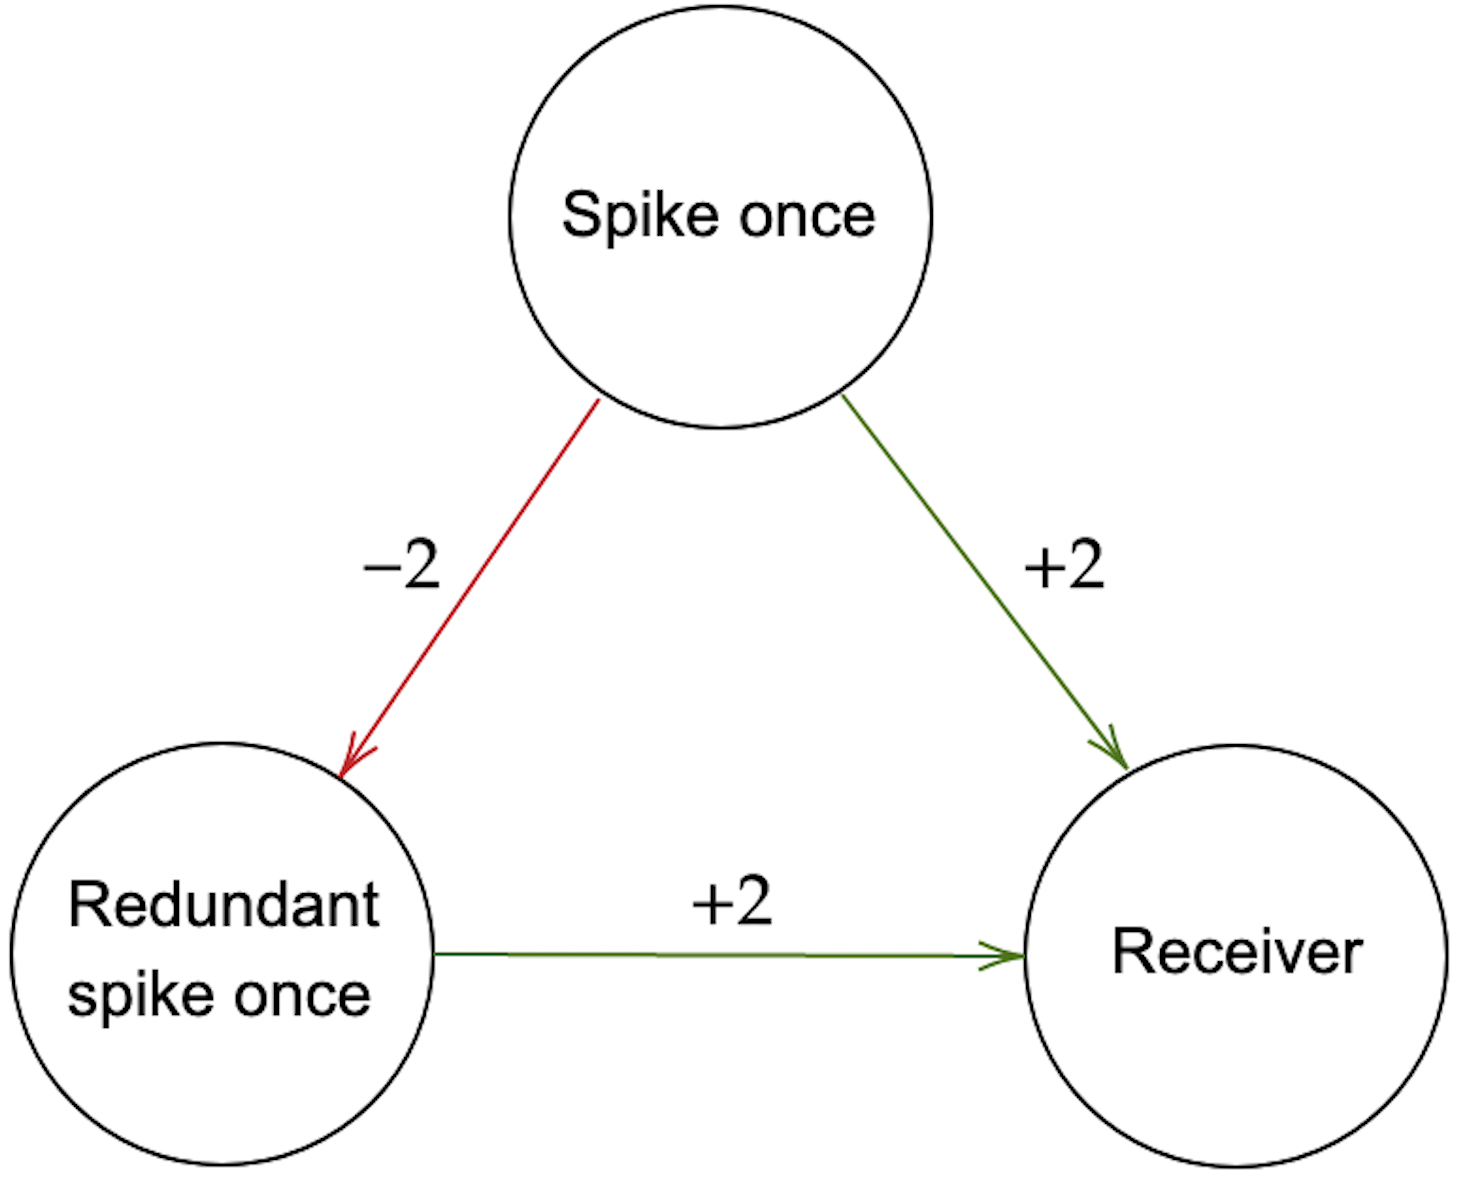
\includegraphics[width=.5\linewidth]{latex/Images/brain_adaptation_alternative.png}
%    \caption{Alternative neural pathway for a redundancy of the spike\_once neuron. If the spike\_once neuron dies due to simulated radiation-induced SEEs ($vth=inf$), the redundancy neuron inhibition is eliminated. Without inhibition, the redundant spike\_once neuron copies the spike\_once behaviour with a delay of 1 timestep.}
%    \label{fig:eg_brain_adaptation}
%\end{figure}
\begin{rudifig}{0.5\hsize}{Fig. 3: Redundancy}
    %\hspace{2em}
%\begin{rudifig}{Fig. 3: Redundancy}
    %
\includegraphics[width=\hsize]{ru_en_1}
    %\hspace{-1em}
    %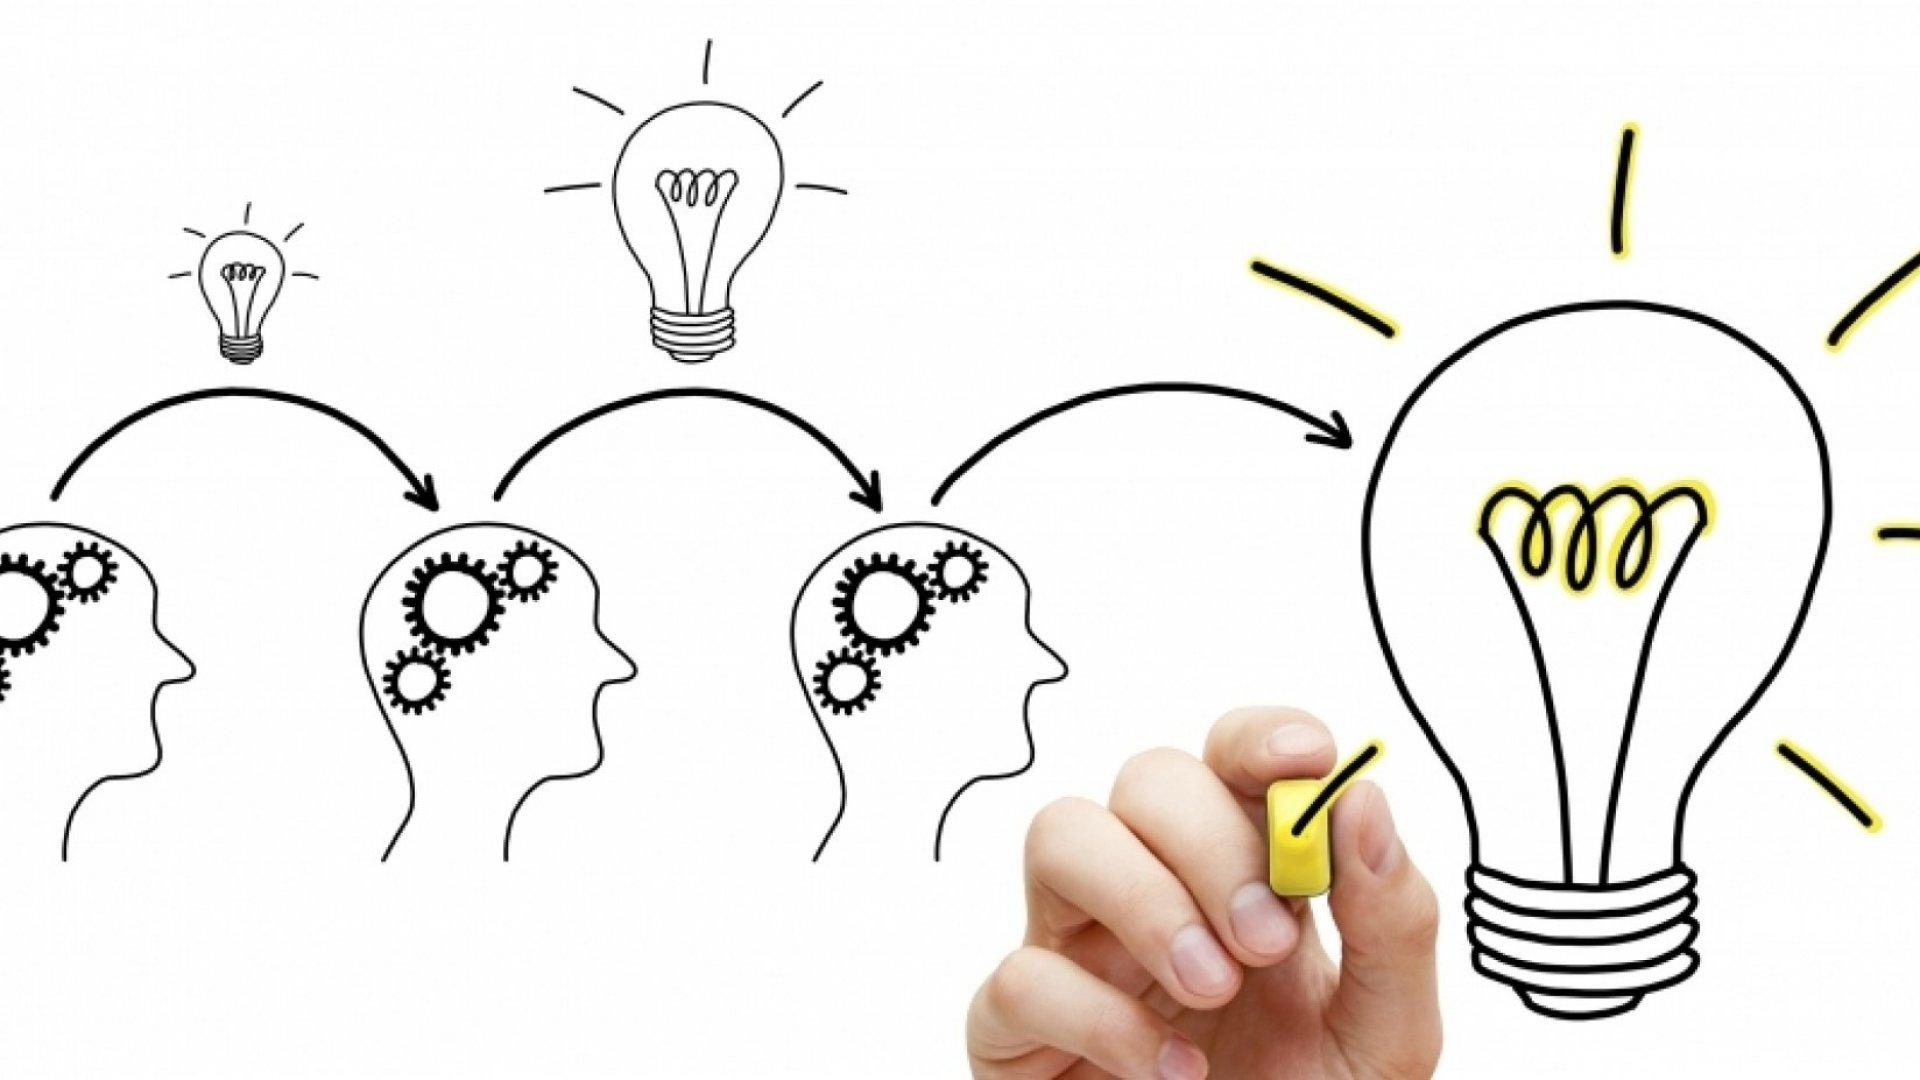
\includegraphics[width=700pt]{latex/Images/os0.jpg}
    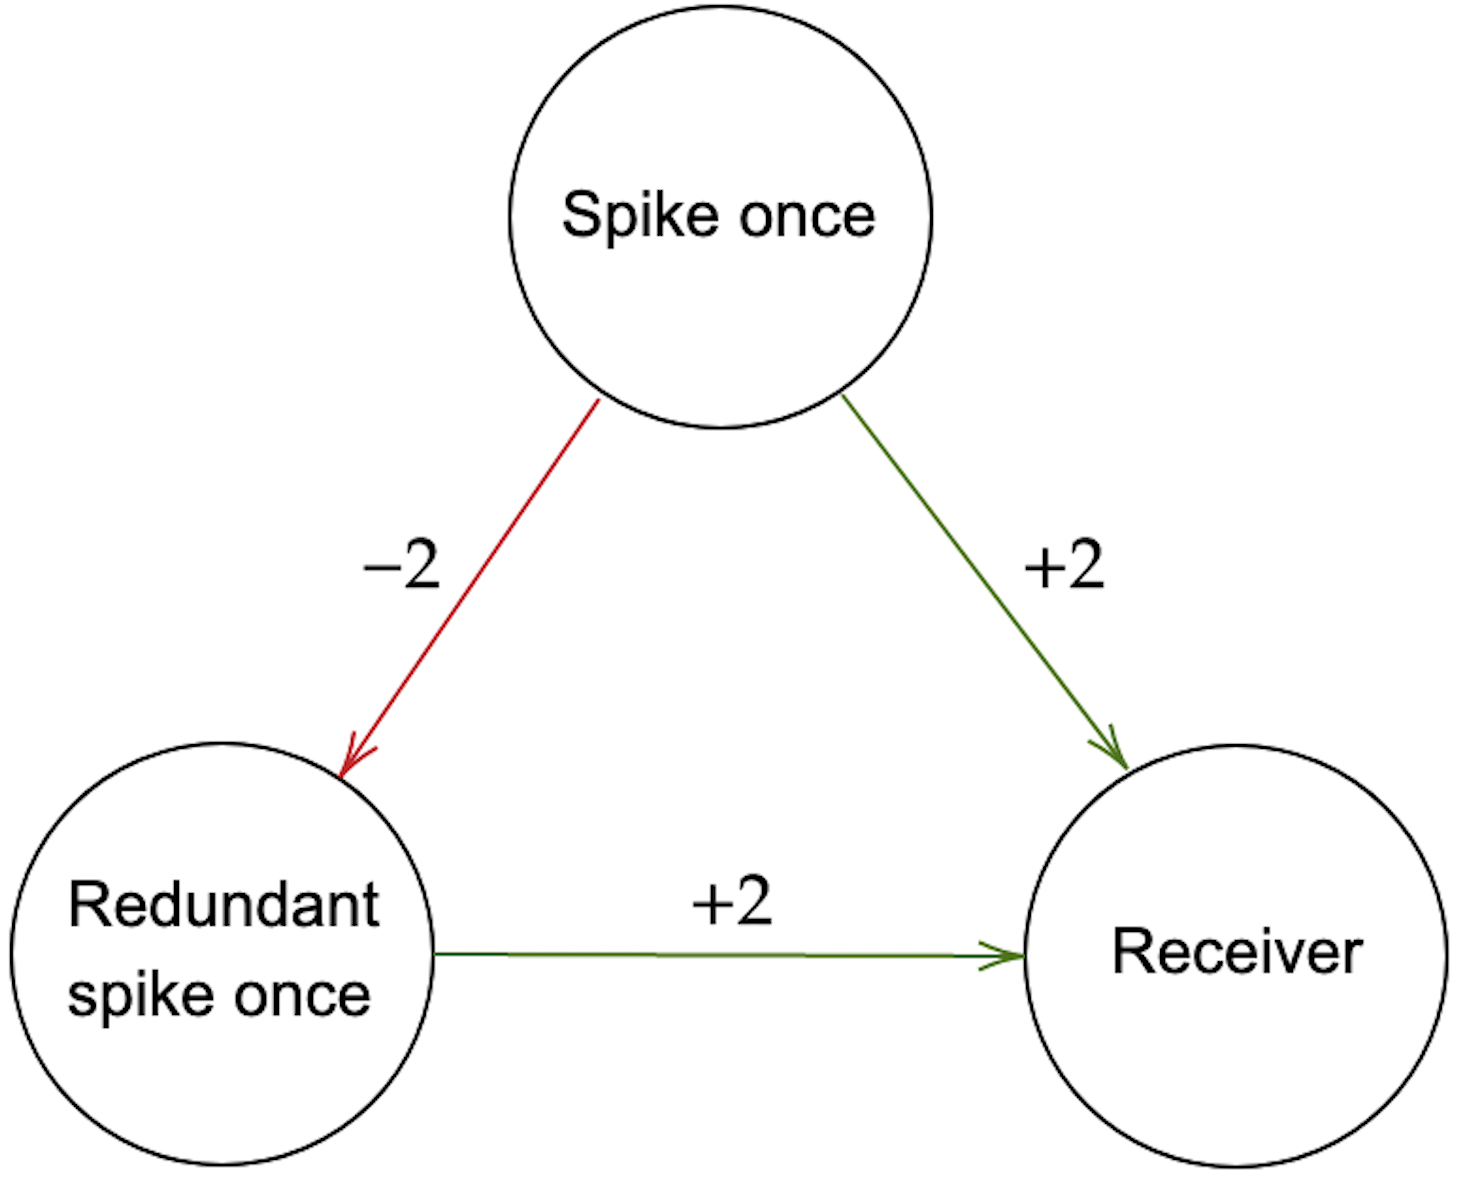
\includegraphics[width=1\linewidth]{latex/Images/brain_adaptation_alternative.png}
    %\caption{Alternative neural pathway for a redundancy of the spike\_once neuron. If the spike\_once neuron dies due to simulated radiation-induced SEEs ($vth=inf$), the redundancy neuron inhibition is eliminated. Without inhibition, the redundant spike\_once neuron copies the spike\_once behaviour with a delay of 1 timestep.}
    \label{fig:eg_brain_adaptation}
\end{rudifig}


\vspace{-15em}


}
\colchunk[2]{%
    \begin{rudifig}{1\hsize}{Fig. 2: Output SNN}
        %\vspace{-3em}
            %\hspace{-1em}
            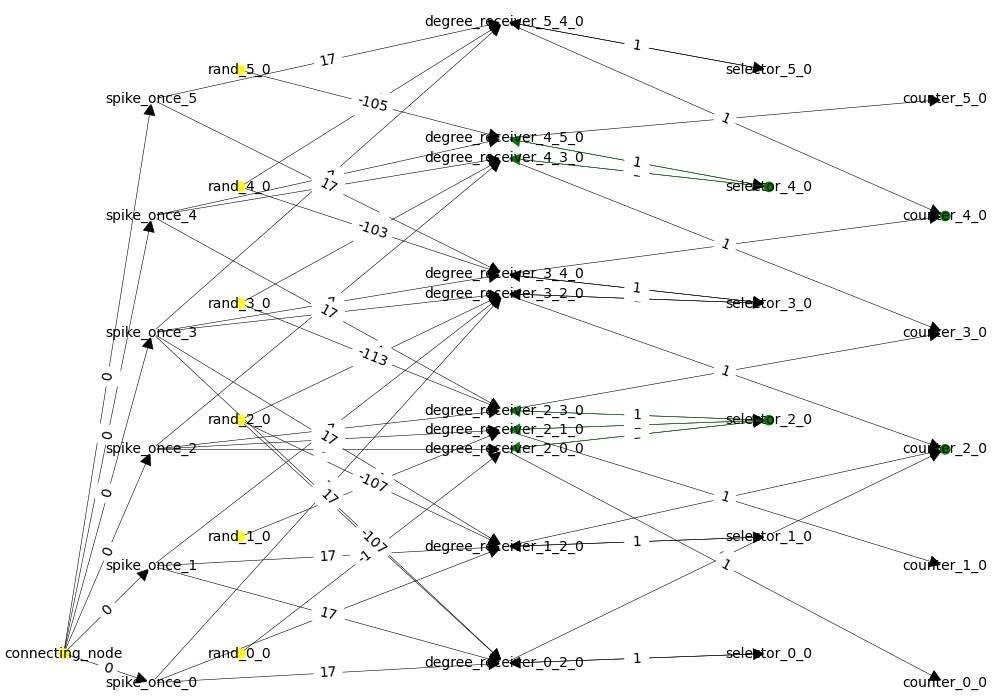
\includegraphics[width=1.\linewidth]{latex/Images/cropped.jpeg}
            %\caption{Example SNN encoding of algorithm to approximate MDS on the input graph of \cref{fig:input_graph}. This module is connected in series where the mark counter neuron takes up the role of spike\_once neuron in the next round of the approximation algorithm. For a more detailed description of the SNN implementation the reader is referred to Diehl et al. \cite{diehl}. %TODO: update to match updated input graph.
            %}
            \label{fig:encoded_snn}
        \end{rudifig}
        
        
        
\begin{rudifig}{1\hsize}{Fig. 4: Adaptation: Redundancy (And Radiation in Red)}
    %\hspace{-1.5em}
    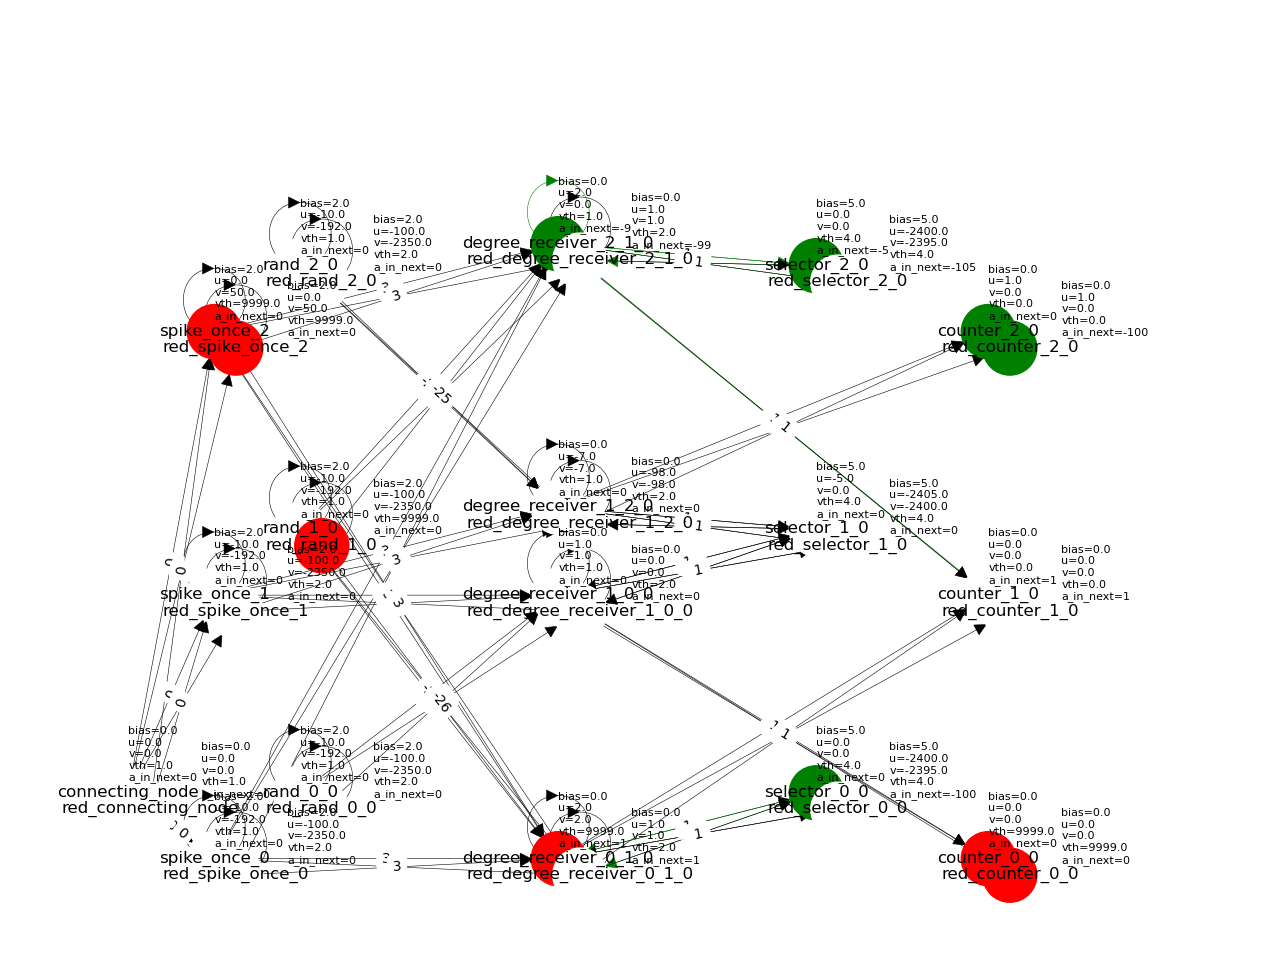
\includegraphics[width=1\linewidth]{latex/Images/rad_adapted.png}
    %\caption{Example SNN encoding of algorithm to approximate MDS on the input graph of \cref{fig:input_graph}. This module is connected in series where the mark counter neuron takes up the role of spike\_once neuron in the next round of the approximation algorithm. For a more detailed description of the SNN implementation the reader is referred to Diehl et al. \cite{diehl}. %TODO: update to match updated input graph.
    %}
    \label{fig:encoded_snn}
\end{rudifig}


}
        \else
            % Local compilation
            %\section{Methodology}\label{sec:methodology}
\colchunk[1]{%
        %EDUCATION\\*
        %\\*[.5\baselineskip]
        %\\*
%\titlespacing*{\subsection}{1pt}{1.1\baselineskip}{\baselineskip}        
\vspace{-40em}
\section{Select Distributed Algorithm}\label{subsec:algorithm}
The Minimum Dominating Set Approximation algorithm as presented by Alipour et al., is specified as:
%Within the graph algorithms, some SNN algorithms may be naturally more robust than others. For example, SNN algorithms that calculate the shortest path within graphs may automatically re-route if radiation imposed neuron-death occurs. However, since this research aims at determining the effectivity of brain adaptation mechanisms, a stricter test is found in algorithms that can fail to produce meaningful output if a single neuronal or synaptic property is changed. Therefore, 
%\begin{algorithm}%[h]%[1]
    %\caption{Distributed Algorithm for computing a total dominating set in a graph with given integer $m\geq 0$.}\label{alg:alipour}

%\KwData*
\textbf{Input:}\textit{Connected, planar, triangle-free graph of size $n$.}\\
%\KwResult*{\textit{Set of nodes that form a minimum total dominating set.}}
\textbf{Output:}\textit{Set of nodes that form a minimum total dominating set.}\\
%\setlist{nolistsep}
\vspace{-1.5em}
\begin{enumerate}[noitemsep]
\itemsep-1.5em
\item \textit{In the first round, each node $v_i$ chooses a random number $0<r_i<1$, computes degree $d_i$ and computes its weight $w_i=d_i+r_i$ and sends $w_i$ to its adjacent neighbours.}\\
\item \textit{In the second round, each node $v$ marks a neighbour vertex $v_i$ whose weight $w_i$ is maximum among all the other neighbours of $v$.}\\
\For{$m$ rounds}{
    \begin{enumerate}[noitemsep]
        \itemsep-1.5em
    \item \textit{Let $x_i$ be the number of times that a vertex is marked by its neighbour vertices, let $w_i=x_i+r_i$}\\
    \item \textit{Unmark the marked vertices.}\\
    \item \textit{Each vertex marks the vertex with maximum $w_i$ among its neighbour vertices.}\\
    \end{enumerate}
}
\vspace{1.5em}
\item \textit{The marked vertices are considered as the vertices in our total dominating set for $G$.}
\end{enumerate}
%\end{algorithm}

\section{Convert Algorithm to Spiking Neural Network(SNN)}\label{subsec:algo_to_snn}
%\vspace{-1.5em}
Next, an SNN implementation of this algorithm is generated using Leaky-Integrate-and-Fire (LIF) neurons. This implementation takes as input connected, triangle-free, planar graphs (E.g. Fig 1.). Then it converts these graphs into the specification of an SNN that is encoded in a new graph (E.g. Fig 2.). These graphs can then be simulated using the Lava backend by Loihi, or a custom Networkx SSN simulator backend.

\section{Apply Adaptation Mechanism to SNN}\label{subsec:adaptation}
The SNN is enhanced with redundant neurons, that are by default inhibited by their original neuron (Fig. 3). If the original neuron dies, the redundant neuron automatically takes over. 


\section{Simulate Radiation on SNN}\label{subsec:}
Space radiation damage is simulated in the form of random neuron deaths. Redundant neurons can die too (see red neuron pairs in Fig 4).. \vspace{-7em}
\section{Compare SNN Performance With-/out Adaptation}\label{subsec:}
%Algorithm performance during simulated radiation exposure, is compared with/without the adaptation mechanism.\\
SNN performance during simulated radiation exposure is compared with/without adaptation.\\
%\\*[.5\baselineskip]
\\*
%\begin{figure}[]
%    \centering
%    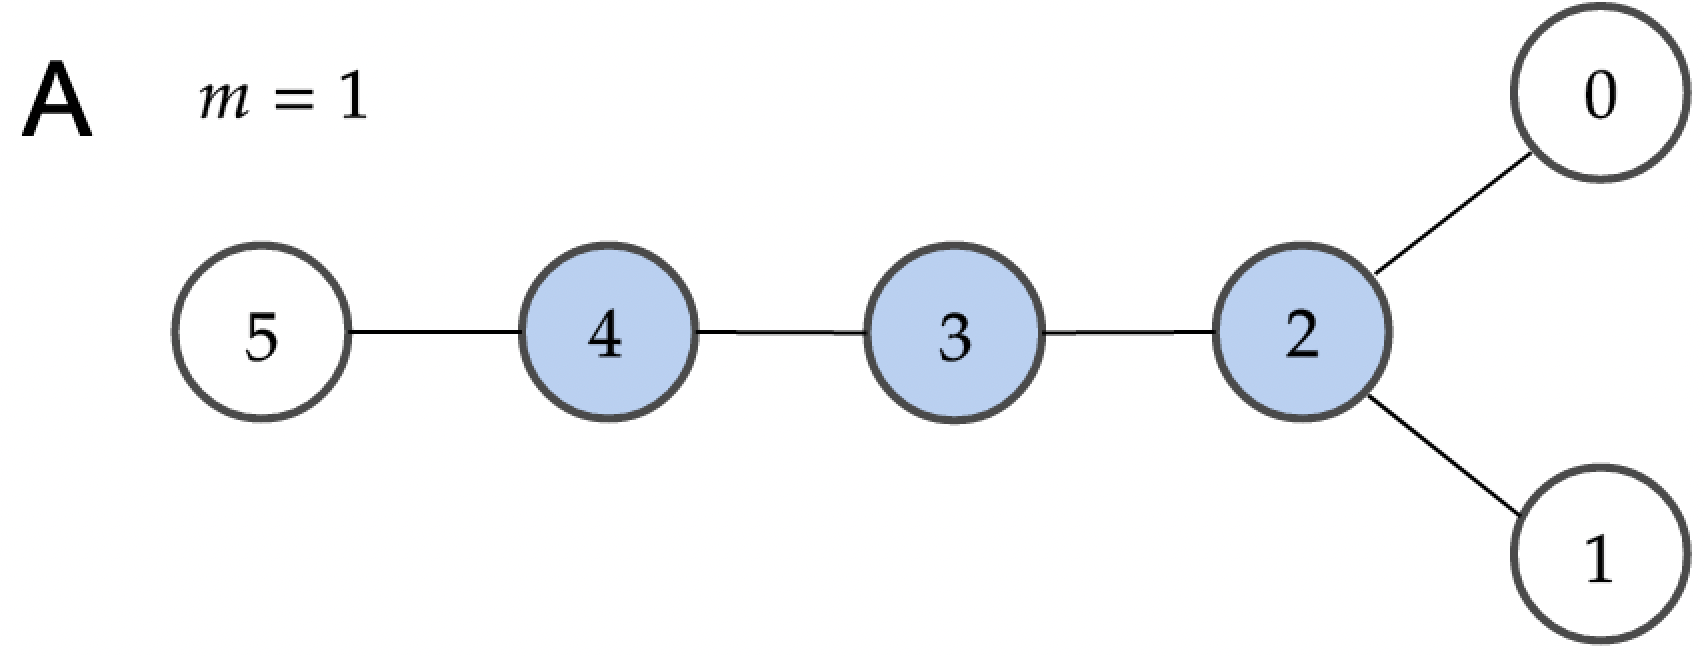
\includegraphics[width=8cm]{latex/Images/input_graph_G_6_0_alternative1.png}
%    \caption{Example input graph. For $m=1$ the algorithm still selects 3 nodes as it is an approximation of the MDS.}
%    \label{fig:input_graph}
%\end{figure}
%\hspace{-3em}
\vspace{-45em}
\begin{rudifig}{0.49\hsize}{Fig. 1: Input Graph}
%\begin{rudifig}{Fig. 1: Input Graph}
    \hspace{-1.5em}
    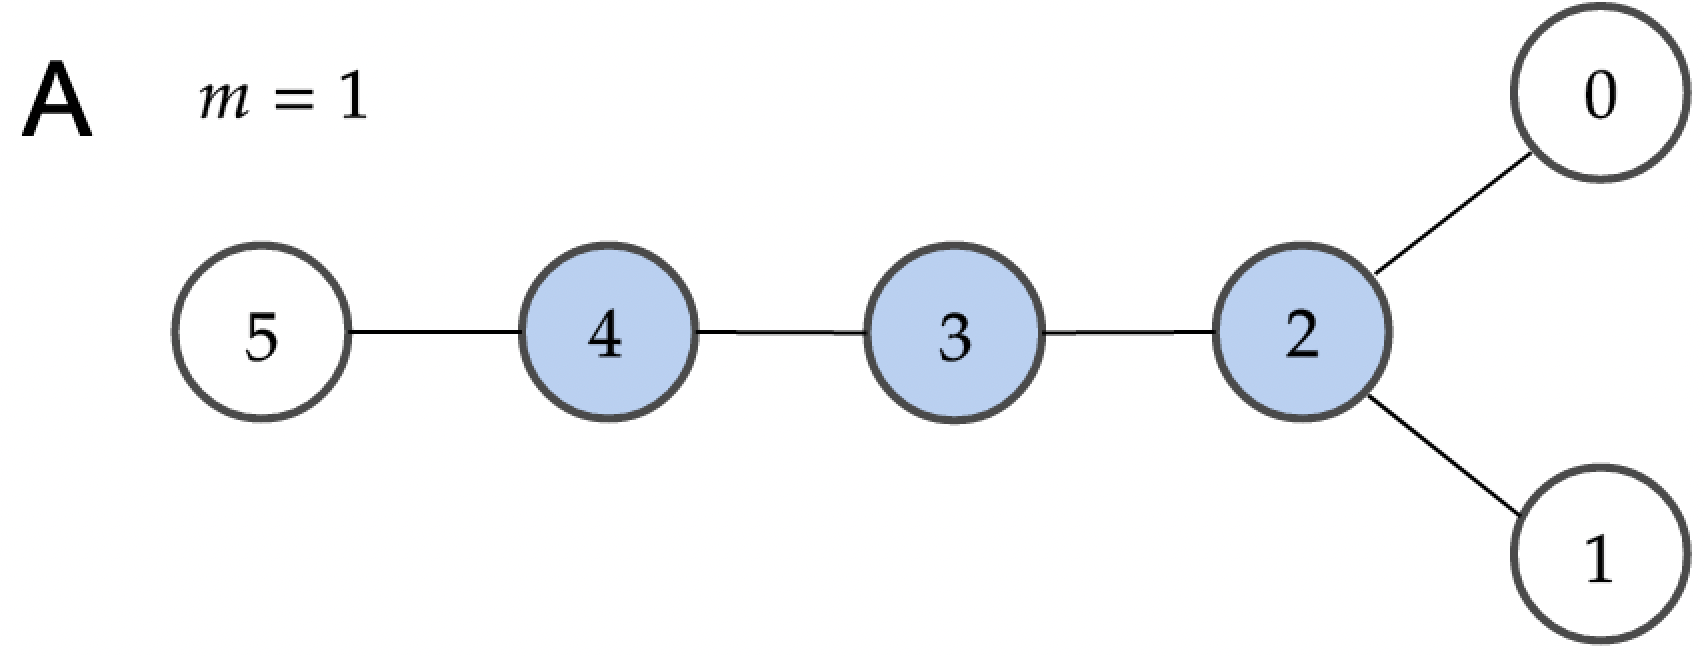
\includegraphics[width=1.1\linewidth]{latex/Images/input_graph_G_6_0_alternative1.png}
    %\caption{Example input graph. For $m=1$ the algorithm still selects 3 nodes as it is an approximation of the MDS.}
    \label{fig:input_graph}
\end{rudifig}
% Non poster image:
%\begin{figure}[H]
%    \centering
%    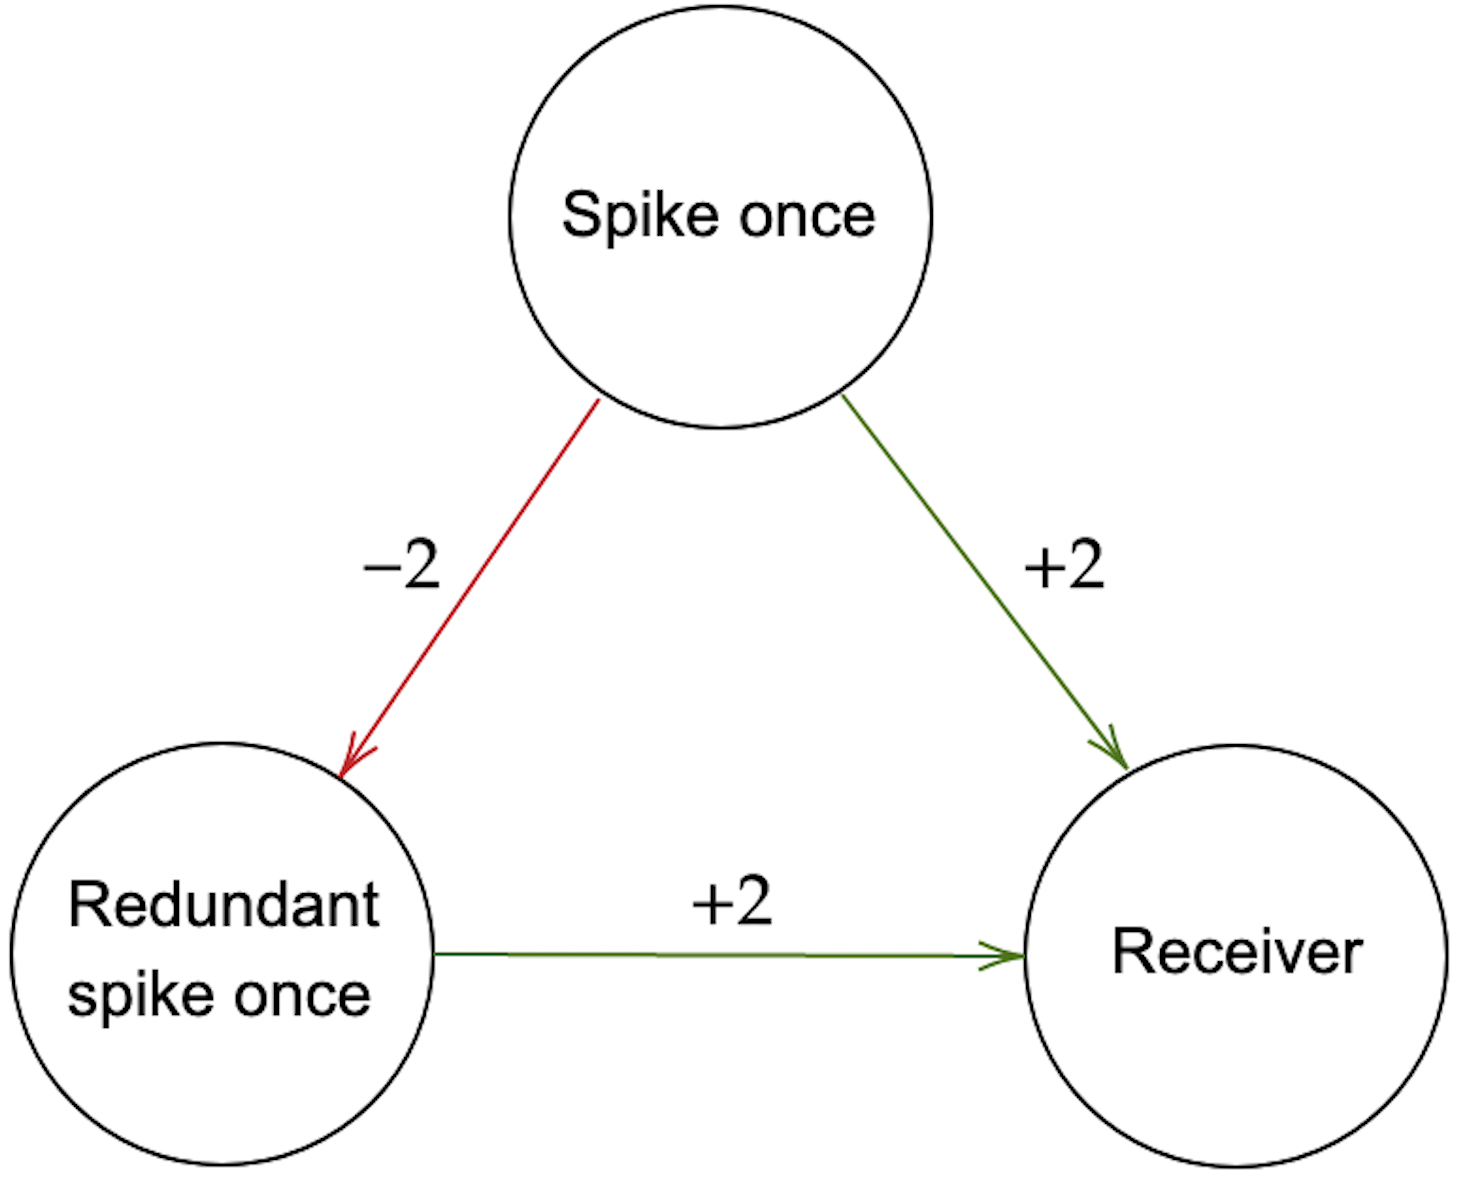
\includegraphics[width=.5\linewidth]{latex/Images/brain_adaptation_alternative.png}
%    \caption{Alternative neural pathway for a redundancy of the spike\_once neuron. If the spike\_once neuron dies due to simulated radiation-induced SEEs ($vth=inf$), the redundancy neuron inhibition is eliminated. Without inhibition, the redundant spike\_once neuron copies the spike\_once behaviour with a delay of 1 timestep.}
%    \label{fig:eg_brain_adaptation}
%\end{figure}
\begin{rudifig}{0.5\hsize}{Fig. 3: Redundancy}
    %\hspace{2em}
%\begin{rudifig}{Fig. 3: Redundancy}
    %
\includegraphics[width=\hsize]{ru_en_1}
    %\hspace{-1em}
    %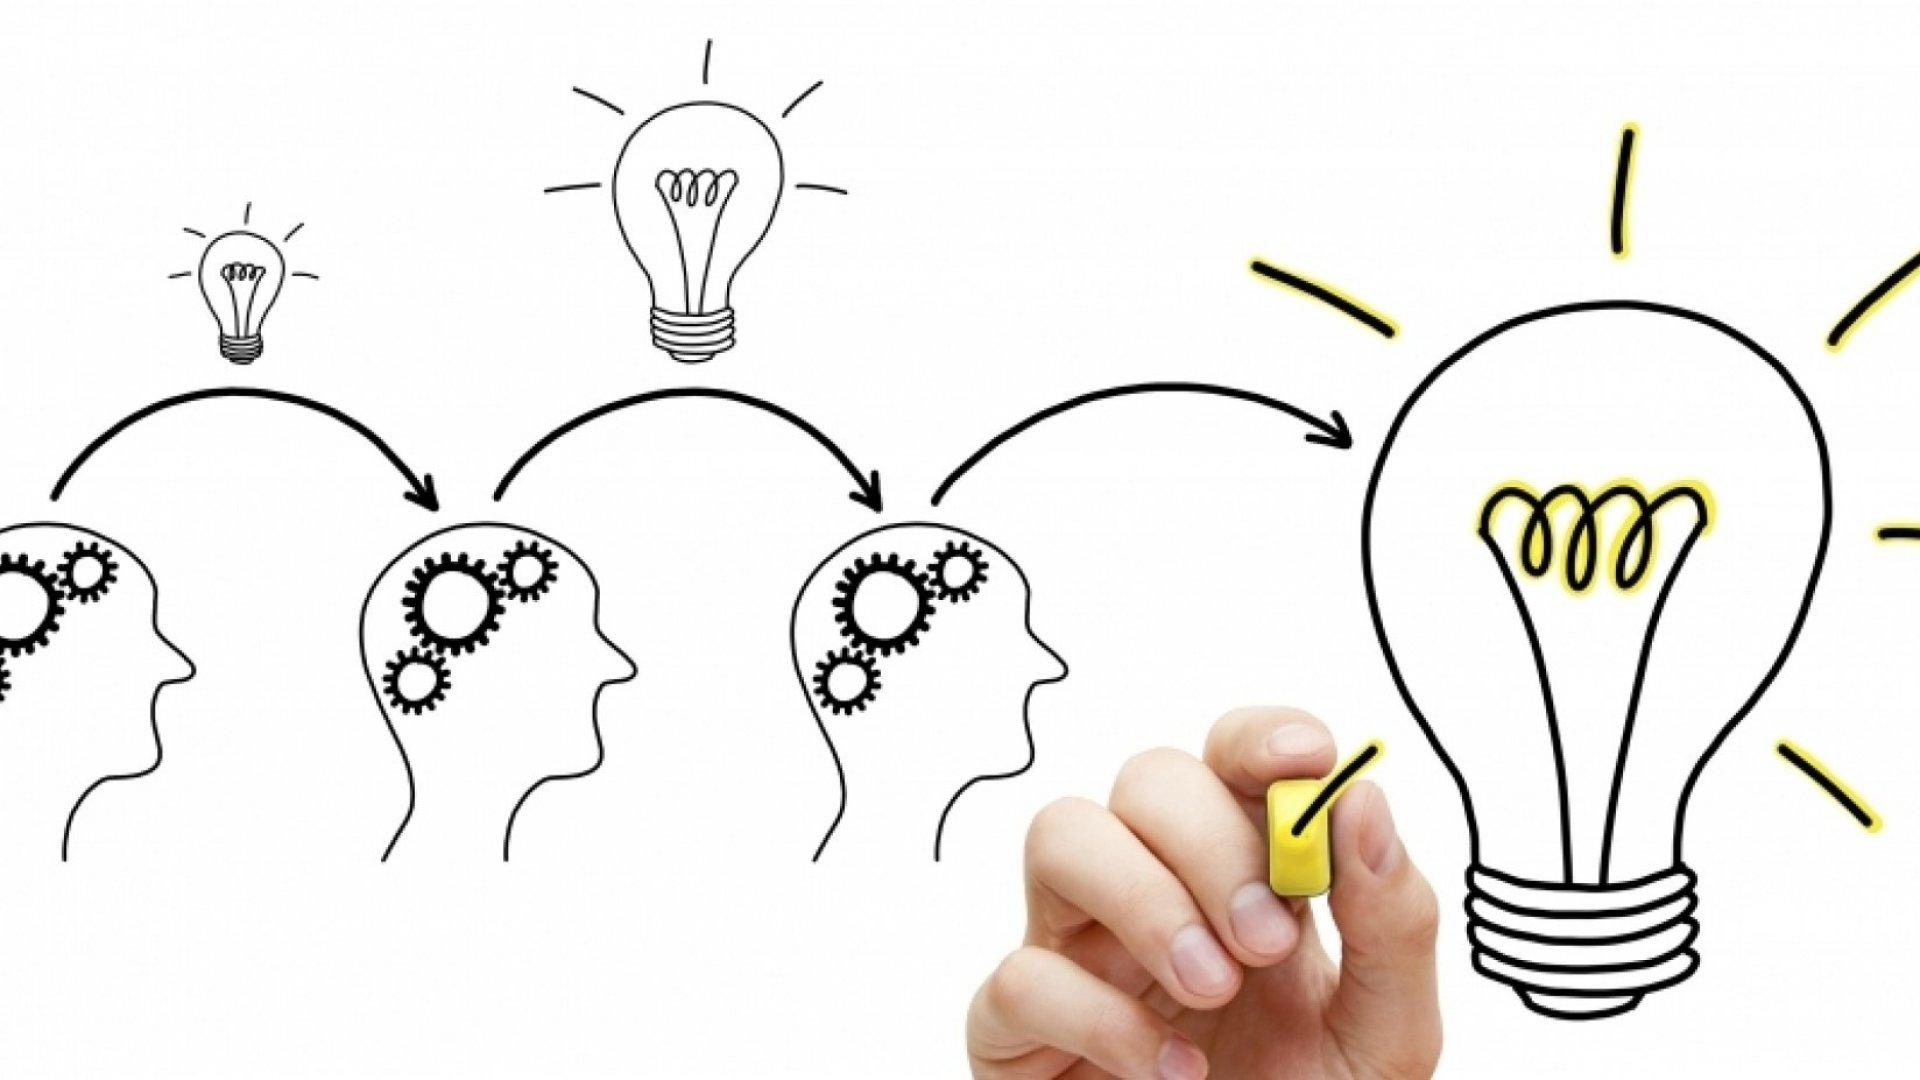
\includegraphics[width=700pt]{latex/Images/os0.jpg}
    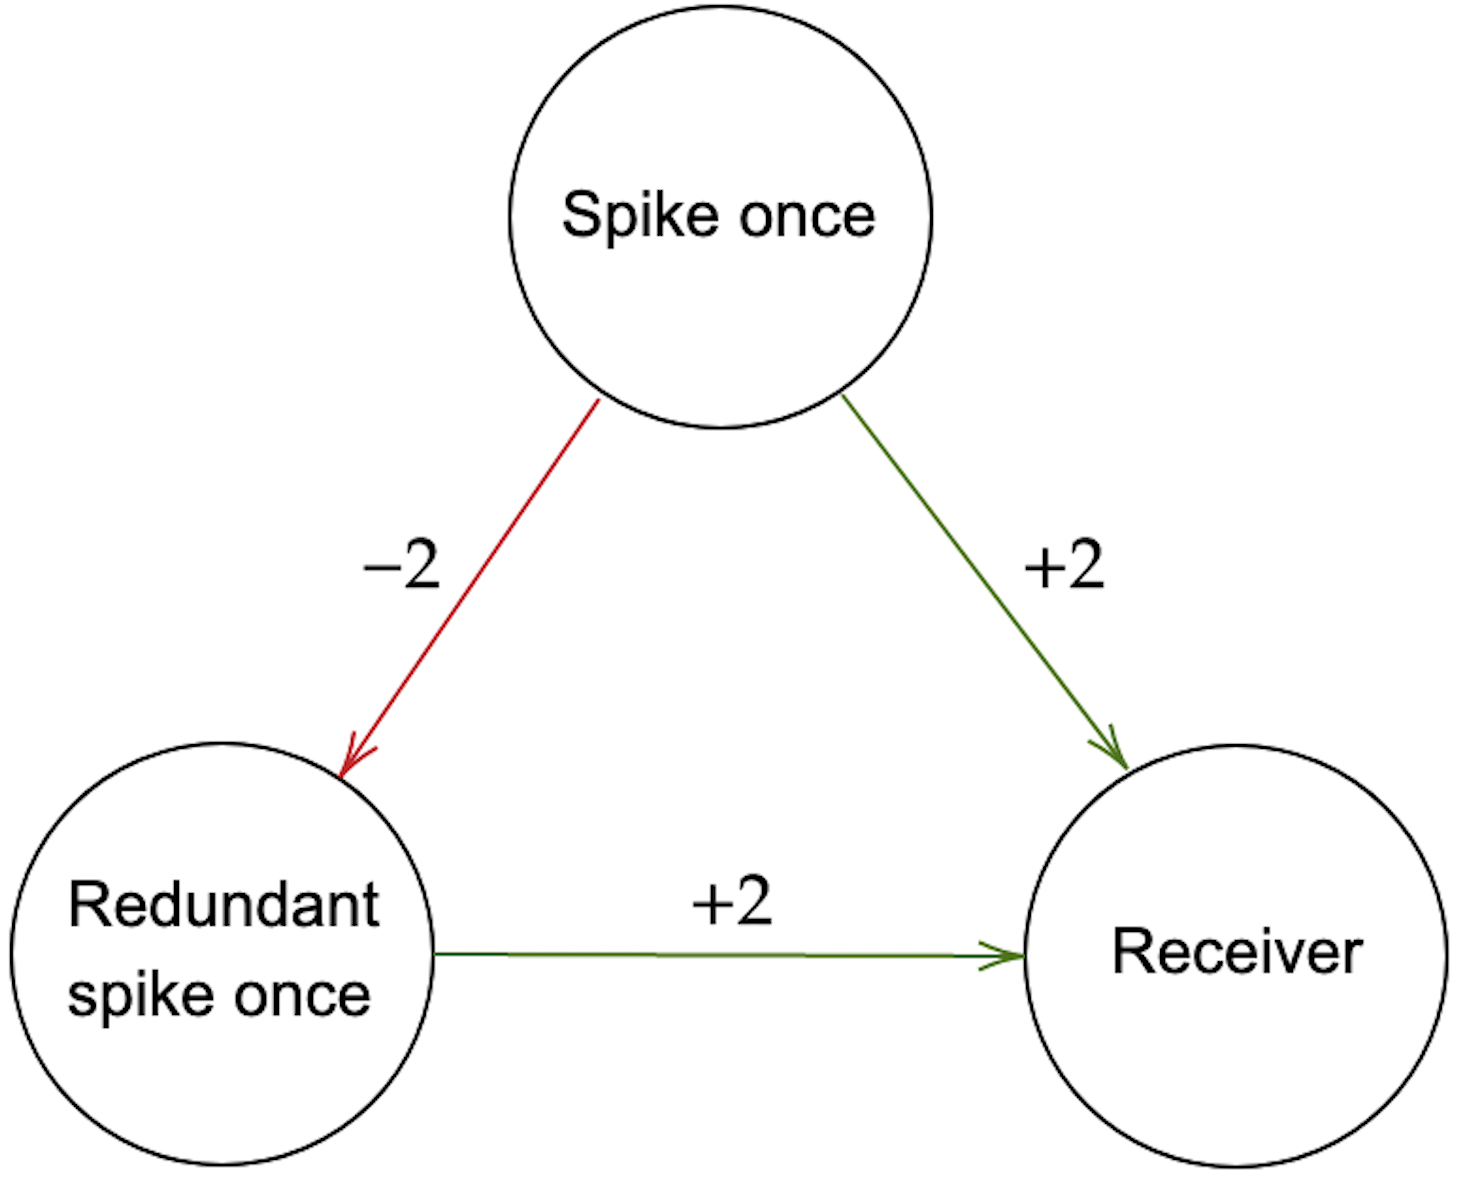
\includegraphics[width=1\linewidth]{latex/Images/brain_adaptation_alternative.png}
    %\caption{Alternative neural pathway for a redundancy of the spike\_once neuron. If the spike\_once neuron dies due to simulated radiation-induced SEEs ($vth=inf$), the redundancy neuron inhibition is eliminated. Without inhibition, the redundant spike\_once neuron copies the spike\_once behaviour with a delay of 1 timestep.}
    \label{fig:eg_brain_adaptation}
\end{rudifig}


\vspace{-15em}


}
\colchunk[2]{%
    \begin{rudifig}{1\hsize}{Fig. 2: Output SNN}
        %\vspace{-3em}
            %\hspace{-1em}
            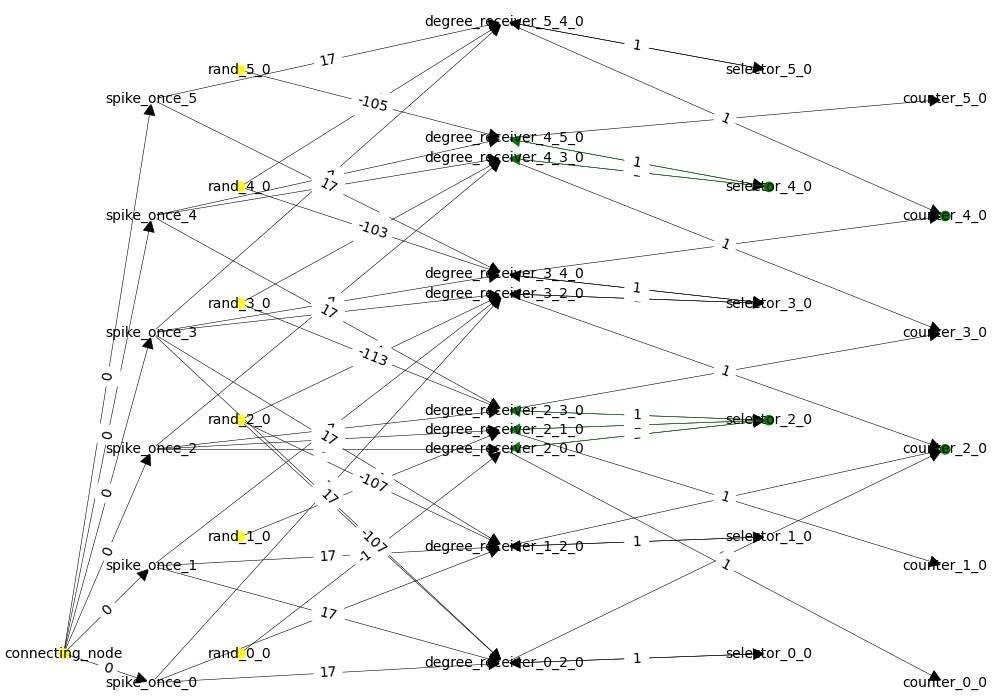
\includegraphics[width=1.\linewidth]{latex/Images/cropped.jpeg}
            %\caption{Example SNN encoding of algorithm to approximate MDS on the input graph of \cref{fig:input_graph}. This module is connected in series where the mark counter neuron takes up the role of spike\_once neuron in the next round of the approximation algorithm. For a more detailed description of the SNN implementation the reader is referred to Diehl et al. \cite{diehl}. %TODO: update to match updated input graph.
            %}
            \label{fig:encoded_snn}
        \end{rudifig}
        
        
        
\begin{rudifig}{1\hsize}{Fig. 4: Adaptation: Redundancy (And Radiation in Red)}
    %\hspace{-1.5em}
    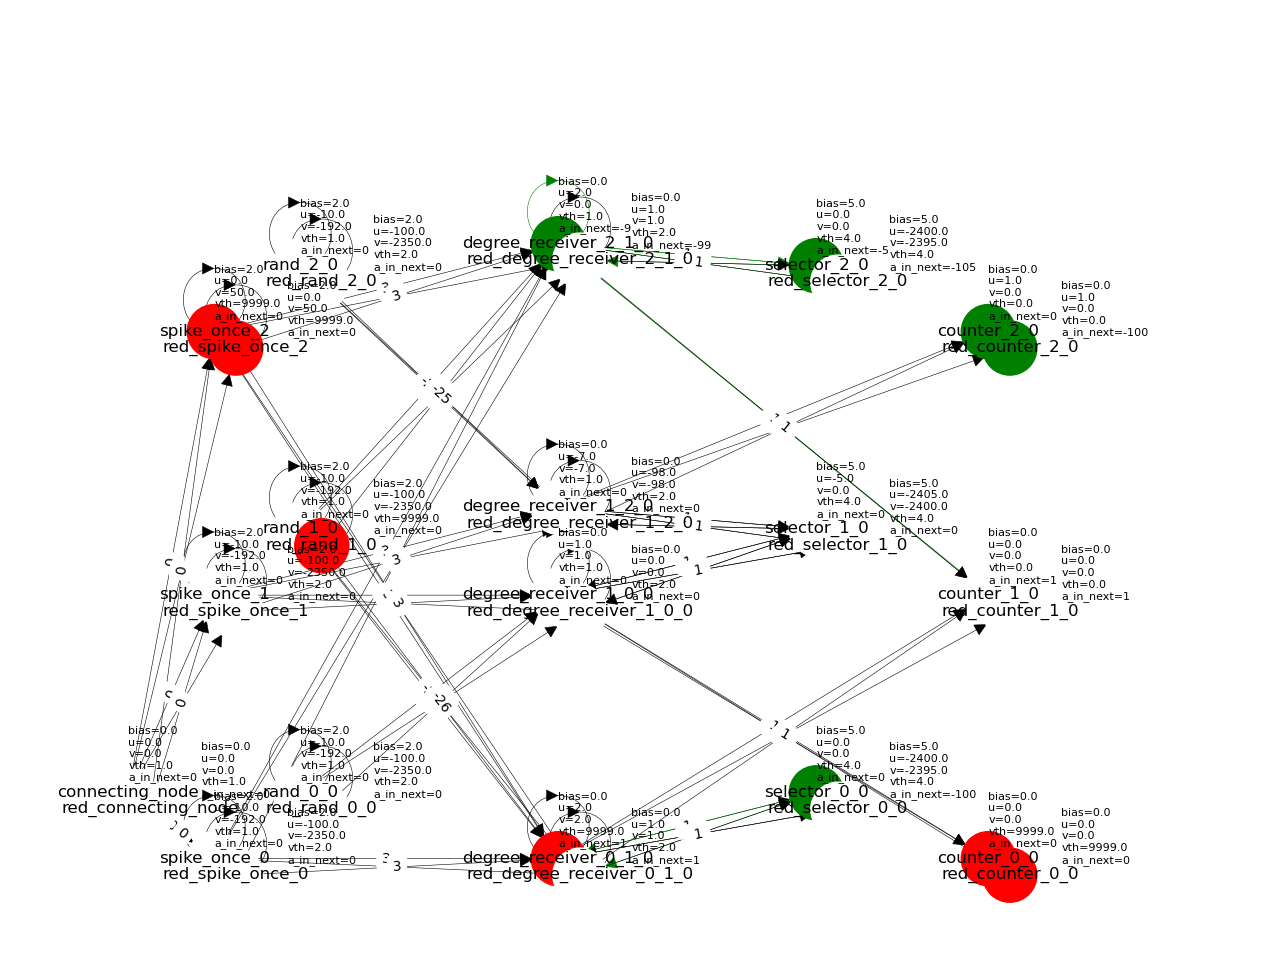
\includegraphics[width=1\linewidth]{latex/Images/rad_adapted.png}
    %\caption{Example SNN encoding of algorithm to approximate MDS on the input graph of \cref{fig:input_graph}. This module is connected in series where the mark counter neuron takes up the role of spike\_once neuron in the next round of the approximation algorithm. For a more detailed description of the SNN implementation the reader is referred to Diehl et al. \cite{diehl}. %TODO: update to match updated input graph.
    %}
    \label{fig:encoded_snn}
\end{rudifig}


}
        \fi
    \end{multicols}
\end{rudiblockiintroduction}

%%\begin{rudiblockimethodsresultsbody}
%%    \begin{multicols}{3}
%%    \end{rudisubblock}
%%\end{rudiblockimethodsresultsbody}

% ======================================================================

\begin{rudiblockconclusion}
    \begin{multicols}{3}
        \ifx\homepath\overleafhome
            % Overleaf compilation.
            %\section{Results \& Discussion}\label{sec:results}
%\textcolor{red}{TODO: change dummy results with actual results.}
%\textcolor{red}{TODO: Include synaptic death.}
%The domains specified in \cref{subsec:results_energy_consumption} to \cref{subsec:results_radiation_robustness} are evaluated as part of the presentation of the results of this experiment. The first three are used to put the radiation robustness in perspective. All four domains are compared to the reference baseline presented in \cref{sec:methodology}.
\subsection*{Radiation Robustness}\label{subsec:algorithm_performance}

\begin{table}[H]
\caption{Average fraction of correct outputs of the SNN implementation with and without adaptation. Neuron deaths can occur in default and redundant LIF neurons.}
\begin{tabular}{llllll}
        & \multicolumn{5}{l}{Neuron Death Percentage in SNN} \\ \cmidrule{2-6}
        Adaptation & 0\%   5\% & 10\%    & 25\%     \\ \hline
        Without      & 1 &  1    & 0                 \\
        With      & 1 & 1    & 0.5                   \\    
\end{tabular}
\end{table}

%If  multiple brain adaptation mechanisms are implemented before the deadline, use line type to distinguish between these implementations, and generate 3 plots, or use line colour to distinguish between redundancy levels. (Depending on what is most insightful).

\subsection*{Neuronal, Synaptic \& Energy Costs}\label{subsec:results_neuronal_synaptic_overcapacity}
%By taking this factor into account, a context can be provided for the added value of using brain-inspired radiation robustness implementations in neuromorphic hardware.

\begin{table}[H]
\caption{The multiple of the amount of neurons and synapses used by adaptation implementation, compared to the default SNN implementation.}\label{tab:overcapacity}
\begin{tabular}{llll}
           & \multicolumn{3}{l}{Average Cost of Adaptation Mechanism} \\ \cmidrule{2-4}
           Graph Size & Neuronal     & Synaptic & Spikes                   \\ \hline 
3       & 5.7          & 8.3        & 32                \\
4      & 5.8            & 10        & 37.5                  \\
5      & 5.8            & 10.2           & 64              
\end{tabular}
\end{table}\vspace{-1em}
Note this is the average overcapacity for $m=0$ and $m=1$ combined.
%\subsection*{}\label{subsec:results_energy_consumption}
%\begin{table}[H]
%\caption{Fraction of additional spikes consumed by adaptation mechanism.}
%\begin{tabular}{llllll}
%           & \multicolumn{5}{l}{Neuron Death Percentage in SNN.} \\ %\cmidrule{2-6} % Neuron Death in SNN: with/ without adaption%
%          Graph Size & 0\%    & 10\%    & 25\%    & 50\% \\ \hline
%3      & 32    & 4     & 4       & 4             \\
%4      & 37.5      & 4       & 4       & 4            \\
%5      & 4      & 4       & 4       & 4          
%\end{tabular}
%\end{table}
%Note this is the average overcapacity for $m=0$ and $m=1$ combined.
%\textit{Depending on the radiation test method, the energy consumption may be monitored hardwarematically, or estimated softwarematically. This may be challenging in the case of reliance on neuromorphic cloud architectures for testing, as some may not provide the ability to measure and/or report energy consumption. An approximation to the energy consumption could be counting the occurrence of neuron spikes. This is because neuromorphic architectures are considered to only consume significant amounts of energy when they spike.}

%\subsection*{Time Complexity}\label{subsec:time_complexity}
%TODO:Presents the time complexity of the default SNN as two terms: network initialisation and network runtime. Then presents the same parameters for the adapted SNN. If relevant, as a function of the level of redundancy.

%\subsection*{Space Complexity}\label{subsec:space_complexity}
%TODO:Presents the space complexity of the default SNN as two terms: network initialisation and network runtime. Then presents the same parameters for the adapted SNN. If relevant, as a function of the level of redundancy.

            
\vspace{-2em}\section{Discussion}\label{sec:discussion}
\vspace{-1em}
The reliability of the results can be improved by running the algorithm on more and larger graphs. Running on the Loihi 2 using the Lava 0.4.0 Framework may facilitate this. 

The apparent non-linear growth of the energy consumption in terms of spikes is not expected for the brain adaptation implementation. This is not expected because the redundant neurons should either be inhibited once, or, if they take over from the dead neuron, repeat the exact same spike pattern the dead neuron would have given. This would result in an additive spike increase of roughly the SNN size, not in an exponentially growing multiple. After inspecting the spike behaviour, it is noted that some of the inhibition between neurons and redundant neurons does not stop over time. This causes unneeded spikes generation.

Even though no public SEE propagation mechanisms are known for the Loihi 2 at the time of writing, the representativeness of the simulation can be increased by taking transient effects, synaptic changes, neuron property changes and Von Neumann component malfunctions into account. The current form of redundancy that is implemented is still dependent on particular neuron properties, and no automated method for arbitrary LIF neuron redundancy is presented. A more intelligent adaptation mechanism may allow for a more active neural pathway redirection to realise equivalent robustness levels at a lower neuronal and synaptic overhead. 
%The discussion is used to put the/any radiation robustness differences between using a brain-inspired implementation and regular redundancy in neuromorphic architectures, into perspective. This perspective is generated by discussing the architecture comparison in terms of the characteristics described in \cref{subsec:discussion_performance_trade_off} to \cref{subsec:discussion_space_application_representation_accuracy}.

%\subsection*{Performance Trade-Off}\label{subsec:discussion_performance_trade_off}
%\textit{Increasing the radiation resistance of a default neuromorphic implementation requires some effort. In this study, this effort is realised in the form of a brain-inspired implementation. Such an implementation comes at the cost of resources. In this case those resources are neurons, synapses and energy consumption. Since the comparison is made in terms of radiation robustness, it is important to determine whether it is not merely the consumption of extra resources that led to performance differences. In particular, for space applications, it is important to determine whether the resources that are consumed, for example the energy consumption, are worth the benefits. Each space mission will have its own trade-off in these terms, however, this subsection can shed some light on the trade-off costs. In essence a quantitative insight can be given in terms of performance enhancement and energy cost increases. Similarly, a quantitative insight can be provided in terms of performance enhancement, and the increase in required neurons/synapses and/or hardware mass (if the increase in neurons/synapses require a larger chip).}

%\subsection*{Simulation vs Radiation Testing}
%\textit{If the radiation testing is performed softwarematically in this article submission, this section can be used to convey how portable these results are expected to be to practical radiation tests.}

%\subsection*{Radiation Robustness of Traditional Hardware Elements}
%\textit{The potential bottleneck of traditional Von Neumann hardware elements in neuromorphic hardware, as introduced in \cref{subsec:results_traditional_hardware_element_performance} should be discussed in this section.}

%\subsection*{Space Application Representation Accuracy}\label{subsec:discussion_space_application_representation_accuracy}
%\textit{Some context can be provided in this section to indicate how/up to what extent the radiation testing that is performed for this article submission applies to real space applications.}
% Explain actual space applications may be more AI and less optimisation.

\subsection*{Population Coding}\label{subsec:population_coding}
Other encoding mechanisms than sparse coding may be considered to realise radiation robustness. For example,  in population coding, a population of neurons could be used to represent integer values instead of a single neuron. The \verb+spike_once+ neuron with a synaptic output weight of $x$ could be replaced by $x$ neurons along with $m$ excitatory controller neurons that verify whether each of those neurons is still functional. If part of the population dies, the controller neurons can excite parts of the population to compensate this loss. The $m$ controller neurons could inhibit each other and form a redundancy in the redundancy mechanism.

\subsection*{Rate Coding}\label{subsec:rate_coding}
The first round of the algorithm by Alipour et al. has also been implemented using Lava V0.3.0 using a rate-coding approach, where the numbers are represented as a frequency. No radiation damage simulation has yet been performed on this implementation. However, it is expected that spike frequency modulation can be leveraged to mitigate radiation induced spike loss.

\subsection*{Algorithm Selection}\label{subsec:algorithm_selection}
This work has focussed on a particular optimisation problem, it can be noted that clever algorithm selection (and/or design) for radiation robust SNNs may be used to exchange approximation accuracy for robustness. For example, instead of selecting an algorithm that breaks if a single neuron dies, one could consider shortest-path algorithms that automatically yield a longer path that works around the neuron death. Furthermore, selecting applications that are closer to natural brain functionalities, such as event-based vision, may facilitate brain adaptation mechanisms at a lower cost. For example, in some deep neural networks, neuron death may be a feature instead of a bug, as the retraining phase can in some cases be used to increase the generalisability of the network. % TODO: doubt: is this an example analogous to brain adaptation?

\subsection*{Physical Testing}\label{subsec:physical_testing}
Many of the discussed brain adaptation implementations will fail if the boiler-plate architecture of the SNN suffer from SEEs. This issue can be resolved using fault-tolerance acceptance, redundancy and/or local shielding of boiler-plate architecture components, and by taking boiler-plate SEE propagation mechanisms into account in SNN design. The latter would require physical testing and/or detailed hardware analysis. Industry partners of the Intel Neuromorphic Research Community, such as ESA, NASA and Raytheon are also working on radiation robustness and may be able to share insight in the more detailed radiation effects on the Loihi 2 without incurring export license limitations.
        \else
            % Local compilation
            %\section{Results \& Discussion}\label{sec:results}
%\textcolor{red}{TODO: change dummy results with actual results.}
%\textcolor{red}{TODO: Include synaptic death.}
%The domains specified in \cref{subsec:results_energy_consumption} to \cref{subsec:results_radiation_robustness} are evaluated as part of the presentation of the results of this experiment. The first three are used to put the radiation robustness in perspective. All four domains are compared to the reference baseline presented in \cref{sec:methodology}.
\subsection*{Radiation Robustness}\label{subsec:algorithm_performance}

\begin{table}[H]
\caption{Average fraction of correct outputs of the SNN implementation with and without adaptation. Neuron deaths can occur in default and redundant LIF neurons.}
\begin{tabular}{llllll}
        & \multicolumn{5}{l}{Neuron Death Percentage in SNN} \\ \cmidrule{2-6}
        Adaptation & 0\%   5\% & 10\%    & 25\%     \\ \hline
        Without      & 1 &  1    & 0                 \\
        With      & 1 & 1    & 0.5                   \\    
\end{tabular}
\end{table}

%If  multiple brain adaptation mechanisms are implemented before the deadline, use line type to distinguish between these implementations, and generate 3 plots, or use line colour to distinguish between redundancy levels. (Depending on what is most insightful).

\subsection*{Neuronal, Synaptic \& Energy Costs}\label{subsec:results_neuronal_synaptic_overcapacity}
%By taking this factor into account, a context can be provided for the added value of using brain-inspired radiation robustness implementations in neuromorphic hardware.

\begin{table}[H]
\caption{The multiple of the amount of neurons and synapses used by adaptation implementation, compared to the default SNN implementation.}\label{tab:overcapacity}
\begin{tabular}{llll}
           & \multicolumn{3}{l}{Average Cost of Adaptation Mechanism} \\ \cmidrule{2-4}
           Graph Size & Neuronal     & Synaptic & Spikes                   \\ \hline 
3       & 5.7          & 8.3        & 32                \\
4      & 5.8            & 10        & 37.5                  \\
5      & 5.8            & 10.2           & 64              
\end{tabular}
\end{table}\vspace{-1em}
Note this is the average overcapacity for $m=0$ and $m=1$ combined.
%\subsection*{}\label{subsec:results_energy_consumption}
%\begin{table}[H]
%\caption{Fraction of additional spikes consumed by adaptation mechanism.}
%\begin{tabular}{llllll}
%           & \multicolumn{5}{l}{Neuron Death Percentage in SNN.} \\ %\cmidrule{2-6} % Neuron Death in SNN: with/ without adaption%
%          Graph Size & 0\%    & 10\%    & 25\%    & 50\% \\ \hline
%3      & 32    & 4     & 4       & 4             \\
%4      & 37.5      & 4       & 4       & 4            \\
%5      & 4      & 4       & 4       & 4          
%\end{tabular}
%\end{table}
%Note this is the average overcapacity for $m=0$ and $m=1$ combined.
%\textit{Depending on the radiation test method, the energy consumption may be monitored hardwarematically, or estimated softwarematically. This may be challenging in the case of reliance on neuromorphic cloud architectures for testing, as some may not provide the ability to measure and/or report energy consumption. An approximation to the energy consumption could be counting the occurrence of neuron spikes. This is because neuromorphic architectures are considered to only consume significant amounts of energy when they spike.}

%\subsection*{Time Complexity}\label{subsec:time_complexity}
%TODO:Presents the time complexity of the default SNN as two terms: network initialisation and network runtime. Then presents the same parameters for the adapted SNN. If relevant, as a function of the level of redundancy.

%\subsection*{Space Complexity}\label{subsec:space_complexity}
%TODO:Presents the space complexity of the default SNN as two terms: network initialisation and network runtime. Then presents the same parameters for the adapted SNN. If relevant, as a function of the level of redundancy.

            
\vspace{-2em}\section{Discussion}\label{sec:discussion}
\vspace{-1em}
The reliability of the results can be improved by running the algorithm on more and larger graphs. Running on the Loihi 2 using the Lava 0.4.0 Framework may facilitate this. 

The apparent non-linear growth of the energy consumption in terms of spikes is not expected for the brain adaptation implementation. This is not expected because the redundant neurons should either be inhibited once, or, if they take over from the dead neuron, repeat the exact same spike pattern the dead neuron would have given. This would result in an additive spike increase of roughly the SNN size, not in an exponentially growing multiple. After inspecting the spike behaviour, it is noted that some of the inhibition between neurons and redundant neurons does not stop over time. This causes unneeded spikes generation.

Even though no public SEE propagation mechanisms are known for the Loihi 2 at the time of writing, the representativeness of the simulation can be increased by taking transient effects, synaptic changes, neuron property changes and Von Neumann component malfunctions into account. The current form of redundancy that is implemented is still dependent on particular neuron properties, and no automated method for arbitrary LIF neuron redundancy is presented. A more intelligent adaptation mechanism may allow for a more active neural pathway redirection to realise equivalent robustness levels at a lower neuronal and synaptic overhead. 
%The discussion is used to put the/any radiation robustness differences between using a brain-inspired implementation and regular redundancy in neuromorphic architectures, into perspective. This perspective is generated by discussing the architecture comparison in terms of the characteristics described in \cref{subsec:discussion_performance_trade_off} to \cref{subsec:discussion_space_application_representation_accuracy}.

%\subsection*{Performance Trade-Off}\label{subsec:discussion_performance_trade_off}
%\textit{Increasing the radiation resistance of a default neuromorphic implementation requires some effort. In this study, this effort is realised in the form of a brain-inspired implementation. Such an implementation comes at the cost of resources. In this case those resources are neurons, synapses and energy consumption. Since the comparison is made in terms of radiation robustness, it is important to determine whether it is not merely the consumption of extra resources that led to performance differences. In particular, for space applications, it is important to determine whether the resources that are consumed, for example the energy consumption, are worth the benefits. Each space mission will have its own trade-off in these terms, however, this subsection can shed some light on the trade-off costs. In essence a quantitative insight can be given in terms of performance enhancement and energy cost increases. Similarly, a quantitative insight can be provided in terms of performance enhancement, and the increase in required neurons/synapses and/or hardware mass (if the increase in neurons/synapses require a larger chip).}

%\subsection*{Simulation vs Radiation Testing}
%\textit{If the radiation testing is performed softwarematically in this article submission, this section can be used to convey how portable these results are expected to be to practical radiation tests.}

%\subsection*{Radiation Robustness of Traditional Hardware Elements}
%\textit{The potential bottleneck of traditional Von Neumann hardware elements in neuromorphic hardware, as introduced in \cref{subsec:results_traditional_hardware_element_performance} should be discussed in this section.}

%\subsection*{Space Application Representation Accuracy}\label{subsec:discussion_space_application_representation_accuracy}
%\textit{Some context can be provided in this section to indicate how/up to what extent the radiation testing that is performed for this article submission applies to real space applications.}
% Explain actual space applications may be more AI and less optimisation.

\subsection*{Population Coding}\label{subsec:population_coding}
Other encoding mechanisms than sparse coding may be considered to realise radiation robustness. For example,  in population coding, a population of neurons could be used to represent integer values instead of a single neuron. The \verb+spike_once+ neuron with a synaptic output weight of $x$ could be replaced by $x$ neurons along with $m$ excitatory controller neurons that verify whether each of those neurons is still functional. If part of the population dies, the controller neurons can excite parts of the population to compensate this loss. The $m$ controller neurons could inhibit each other and form a redundancy in the redundancy mechanism.

\subsection*{Rate Coding}\label{subsec:rate_coding}
The first round of the algorithm by Alipour et al. has also been implemented using Lava V0.3.0 using a rate-coding approach, where the numbers are represented as a frequency. No radiation damage simulation has yet been performed on this implementation. However, it is expected that spike frequency modulation can be leveraged to mitigate radiation induced spike loss.

\subsection*{Algorithm Selection}\label{subsec:algorithm_selection}
This work has focussed on a particular optimisation problem, it can be noted that clever algorithm selection (and/or design) for radiation robust SNNs may be used to exchange approximation accuracy for robustness. For example, instead of selecting an algorithm that breaks if a single neuron dies, one could consider shortest-path algorithms that automatically yield a longer path that works around the neuron death. Furthermore, selecting applications that are closer to natural brain functionalities, such as event-based vision, may facilitate brain adaptation mechanisms at a lower cost. For example, in some deep neural networks, neuron death may be a feature instead of a bug, as the retraining phase can in some cases be used to increase the generalisability of the network. % TODO: doubt: is this an example analogous to brain adaptation?

\subsection*{Physical Testing}\label{subsec:physical_testing}
Many of the discussed brain adaptation implementations will fail if the boiler-plate architecture of the SNN suffer from SEEs. This issue can be resolved using fault-tolerance acceptance, redundancy and/or local shielding of boiler-plate architecture components, and by taking boiler-plate SEE propagation mechanisms into account in SNN design. The latter would require physical testing and/or detailed hardware analysis. Industry partners of the Intel Neuromorphic Research Community, such as ESA, NASA and Raytheon are also working on radiation robustness and may be able to share insight in the more detailed radiation effects on the Loihi 2 without incurring export license limitations.
        \fi
    \end{multicols}
\end{rudiblockconclusion}

% ======================================================================

\begin{rudiblockipolicyrecommendations}
    \begin{multicols}{3}
        \ifx\homepath\overleafhome
            % Overleaf compilation.
            %\section{Conclusion}\label{sec:conclusion}
% Talk about results.
%The results presented in \cref{sec:results}, along with their critical context described in \cref{sec:discussion} are to be synthesised in this section to provide a clear insight into the benefits and drawbacks of leveraging implementations inspired by principles of brain adaptation in neuromorphic hardware to increase the radiation robustness of these architectures in space applications.
% Talk about discussion
% Mention whether or not it helped.
Brain-inspired adaptation mechanisms may be used in SNN implementations of graph optimisation problems to increase the radiation robustness of neuromorphic space hardware if SEE propagations can lead to neuron death. Creating more intelligent adaptation mechanisms than separate redundant neuronal pathways for each neuron may increase the radiation robustness of graph optimisation applications  in space at a lower neuronal and synaptic cost.
% Don't mention that symmetries in distributed algorithms may also be leveraged in lowering the cost of these brain adaptations. Not a conclusion, not mentioned before, not related to this work.
% TODO: write something about overhead and spike energy.
            %\vspace{-2em}
\section{Future Work}\label{sec:recommendations}
%\vspace{-1em}
%\textit{Recommendations may be generated based on the listed issues in \cref{sec:discussion}. It is foreseeable that dedicated shielding and or redundancy of critical elements of traditional Von Neumann elements in neuromorphic architectures may be advisable, whilst relying on the brain-inspired implementations in SNNs. Another recommendation that may flow out of this research may concern the integration of brain adaptation principles into the design of SNN implementations that yield space application functionalities. Furthermore, a recommendation may be generated regarding a proposed shift in the moment of training, from pre-trained on the ground, to (re-)training after radiation exposure.}
The overarching research project aims to perform physical radiation tests to gain more insight in the practical usefulness of brain-inspired adaptation mechanisms to hedge against radiation damage in neuromorphic space hardware. Since these tests are costly, a more thorough analysis on a broader scope of adaptation mechanisms is proposed. In particular, the population coding and rate coding options will be explored.% \cref{subsec:algorithm_selection} to  \cref{subsec:physical_testing}.
        \else
            % Local compilation
            %\section{Conclusion}\label{sec:conclusion}
% Talk about results.
%The results presented in \cref{sec:results}, along with their critical context described in \cref{sec:discussion} are to be synthesised in this section to provide a clear insight into the benefits and drawbacks of leveraging implementations inspired by principles of brain adaptation in neuromorphic hardware to increase the radiation robustness of these architectures in space applications.
% Talk about discussion
% Mention whether or not it helped.
Brain-inspired adaptation mechanisms may be used in SNN implementations of graph optimisation problems to increase the radiation robustness of neuromorphic space hardware if SEE propagations can lead to neuron death. Creating more intelligent adaptation mechanisms than separate redundant neuronal pathways for each neuron may increase the radiation robustness of graph optimisation applications  in space at a lower neuronal and synaptic cost.
% Don't mention that symmetries in distributed algorithms may also be leveraged in lowering the cost of these brain adaptations. Not a conclusion, not mentioned before, not related to this work.
% TODO: write something about overhead and spike energy.
            %\vspace{-2em}
\section{Future Work}\label{sec:recommendations}
%\vspace{-1em}
%\textit{Recommendations may be generated based on the listed issues in \cref{sec:discussion}. It is foreseeable that dedicated shielding and or redundancy of critical elements of traditional Von Neumann elements in neuromorphic architectures may be advisable, whilst relying on the brain-inspired implementations in SNNs. Another recommendation that may flow out of this research may concern the integration of brain adaptation principles into the design of SNN implementations that yield space application functionalities. Furthermore, a recommendation may be generated regarding a proposed shift in the moment of training, from pre-trained on the ground, to (re-)training after radiation exposure.}
The overarching research project aims to perform physical radiation tests to gain more insight in the practical usefulness of brain-inspired adaptation mechanisms to hedge against radiation damage in neuromorphic space hardware. Since these tests are costly, a more thorough analysis on a broader scope of adaptation mechanisms is proposed. In particular, the population coding and rate coding options will be explored.% \cref{subsec:algorithm_selection} to  \cref{subsec:physical_testing}.
        \fi
    \end{multicols}
\end{rudiblockipolicyrecommendations}


%\begin{paralleltwoblocks}{0.67}
%    \begin{rudiblockipolicyrecommendations}
%        \begin{multicols}{3}
%            \ifx\homepath\overleafhome
%            % Overleaf compilation.
%            
\vspace{-2em}\section{Discussion}\label{sec:discussion}
\vspace{-1em}
The reliability of the results can be improved by running the algorithm on more and larger graphs. Running on the Loihi 2 using the Lava 0.4.0 Framework may facilitate this. 

The apparent non-linear growth of the energy consumption in terms of spikes is not expected for the brain adaptation implementation. This is not expected because the redundant neurons should either be inhibited once, or, if they take over from the dead neuron, repeat the exact same spike pattern the dead neuron would have given. This would result in an additive spike increase of roughly the SNN size, not in an exponentially growing multiple. After inspecting the spike behaviour, it is noted that some of the inhibition between neurons and redundant neurons does not stop over time. This causes unneeded spikes generation.

Even though no public SEE propagation mechanisms are known for the Loihi 2 at the time of writing, the representativeness of the simulation can be increased by taking transient effects, synaptic changes, neuron property changes and Von Neumann component malfunctions into account. The current form of redundancy that is implemented is still dependent on particular neuron properties, and no automated method for arbitrary LIF neuron redundancy is presented. A more intelligent adaptation mechanism may allow for a more active neural pathway redirection to realise equivalent robustness levels at a lower neuronal and synaptic overhead. 
%The discussion is used to put the/any radiation robustness differences between using a brain-inspired implementation and regular redundancy in neuromorphic architectures, into perspective. This perspective is generated by discussing the architecture comparison in terms of the characteristics described in \cref{subsec:discussion_performance_trade_off} to \cref{subsec:discussion_space_application_representation_accuracy}.

%\subsection*{Performance Trade-Off}\label{subsec:discussion_performance_trade_off}
%\textit{Increasing the radiation resistance of a default neuromorphic implementation requires some effort. In this study, this effort is realised in the form of a brain-inspired implementation. Such an implementation comes at the cost of resources. In this case those resources are neurons, synapses and energy consumption. Since the comparison is made in terms of radiation robustness, it is important to determine whether it is not merely the consumption of extra resources that led to performance differences. In particular, for space applications, it is important to determine whether the resources that are consumed, for example the energy consumption, are worth the benefits. Each space mission will have its own trade-off in these terms, however, this subsection can shed some light on the trade-off costs. In essence a quantitative insight can be given in terms of performance enhancement and energy cost increases. Similarly, a quantitative insight can be provided in terms of performance enhancement, and the increase in required neurons/synapses and/or hardware mass (if the increase in neurons/synapses require a larger chip).}

%\subsection*{Simulation vs Radiation Testing}
%\textit{If the radiation testing is performed softwarematically in this article submission, this section can be used to convey how portable these results are expected to be to practical radiation tests.}

%\subsection*{Radiation Robustness of Traditional Hardware Elements}
%\textit{The potential bottleneck of traditional Von Neumann hardware elements in neuromorphic hardware, as introduced in \cref{subsec:results_traditional_hardware_element_performance} should be discussed in this section.}

%\subsection*{Space Application Representation Accuracy}\label{subsec:discussion_space_application_representation_accuracy}
%\textit{Some context can be provided in this section to indicate how/up to what extent the radiation testing that is performed for this article submission applies to real space applications.}
% Explain actual space applications may be more AI and less optimisation.

\subsection*{Population Coding}\label{subsec:population_coding}
Other encoding mechanisms than sparse coding may be considered to realise radiation robustness. For example,  in population coding, a population of neurons could be used to represent integer values instead of a single neuron. The \verb+spike_once+ neuron with a synaptic output weight of $x$ could be replaced by $x$ neurons along with $m$ excitatory controller neurons that verify whether each of those neurons is still functional. If part of the population dies, the controller neurons can excite parts of the population to compensate this loss. The $m$ controller neurons could inhibit each other and form a redundancy in the redundancy mechanism.

\subsection*{Rate Coding}\label{subsec:rate_coding}
The first round of the algorithm by Alipour et al. has also been implemented using Lava V0.3.0 using a rate-coding approach, where the numbers are represented as a frequency. No radiation damage simulation has yet been performed on this implementation. However, it is expected that spike frequency modulation can be leveraged to mitigate radiation induced spike loss.

\subsection*{Algorithm Selection}\label{subsec:algorithm_selection}
This work has focussed on a particular optimisation problem, it can be noted that clever algorithm selection (and/or design) for radiation robust SNNs may be used to exchange approximation accuracy for robustness. For example, instead of selecting an algorithm that breaks if a single neuron dies, one could consider shortest-path algorithms that automatically yield a longer path that works around the neuron death. Furthermore, selecting applications that are closer to natural brain functionalities, such as event-based vision, may facilitate brain adaptation mechanisms at a lower cost. For example, in some deep neural networks, neuron death may be a feature instead of a bug, as the retraining phase can in some cases be used to increase the generalisability of the network. % TODO: doubt: is this an example analogous to brain adaptation?

\subsection*{Physical Testing}\label{subsec:physical_testing}
Many of the discussed brain adaptation implementations will fail if the boiler-plate architecture of the SNN suffer from SEEs. This issue can be resolved using fault-tolerance acceptance, redundancy and/or local shielding of boiler-plate architecture components, and by taking boiler-plate SEE propagation mechanisms into account in SNN design. The latter would require physical testing and/or detailed hardware analysis. Industry partners of the Intel Neuromorphic Research Community, such as ESA, NASA and Raytheon are also working on radiation robustness and may be able to share insight in the more detailed radiation effects on the Loihi 2 without incurring export license limitations.
%        \else
%            % Local compilation
%            
\vspace{-2em}\section{Discussion}\label{sec:discussion}
\vspace{-1em}
The reliability of the results can be improved by running the algorithm on more and larger graphs. Running on the Loihi 2 using the Lava 0.4.0 Framework may facilitate this. 

The apparent non-linear growth of the energy consumption in terms of spikes is not expected for the brain adaptation implementation. This is not expected because the redundant neurons should either be inhibited once, or, if they take over from the dead neuron, repeat the exact same spike pattern the dead neuron would have given. This would result in an additive spike increase of roughly the SNN size, not in an exponentially growing multiple. After inspecting the spike behaviour, it is noted that some of the inhibition between neurons and redundant neurons does not stop over time. This causes unneeded spikes generation.

Even though no public SEE propagation mechanisms are known for the Loihi 2 at the time of writing, the representativeness of the simulation can be increased by taking transient effects, synaptic changes, neuron property changes and Von Neumann component malfunctions into account. The current form of redundancy that is implemented is still dependent on particular neuron properties, and no automated method for arbitrary LIF neuron redundancy is presented. A more intelligent adaptation mechanism may allow for a more active neural pathway redirection to realise equivalent robustness levels at a lower neuronal and synaptic overhead. 
%The discussion is used to put the/any radiation robustness differences between using a brain-inspired implementation and regular redundancy in neuromorphic architectures, into perspective. This perspective is generated by discussing the architecture comparison in terms of the characteristics described in \cref{subsec:discussion_performance_trade_off} to \cref{subsec:discussion_space_application_representation_accuracy}.

%\subsection*{Performance Trade-Off}\label{subsec:discussion_performance_trade_off}
%\textit{Increasing the radiation resistance of a default neuromorphic implementation requires some effort. In this study, this effort is realised in the form of a brain-inspired implementation. Such an implementation comes at the cost of resources. In this case those resources are neurons, synapses and energy consumption. Since the comparison is made in terms of radiation robustness, it is important to determine whether it is not merely the consumption of extra resources that led to performance differences. In particular, for space applications, it is important to determine whether the resources that are consumed, for example the energy consumption, are worth the benefits. Each space mission will have its own trade-off in these terms, however, this subsection can shed some light on the trade-off costs. In essence a quantitative insight can be given in terms of performance enhancement and energy cost increases. Similarly, a quantitative insight can be provided in terms of performance enhancement, and the increase in required neurons/synapses and/or hardware mass (if the increase in neurons/synapses require a larger chip).}

%\subsection*{Simulation vs Radiation Testing}
%\textit{If the radiation testing is performed softwarematically in this article submission, this section can be used to convey how portable these results are expected to be to practical radiation tests.}

%\subsection*{Radiation Robustness of Traditional Hardware Elements}
%\textit{The potential bottleneck of traditional Von Neumann hardware elements in neuromorphic hardware, as introduced in \cref{subsec:results_traditional_hardware_element_performance} should be discussed in this section.}

%\subsection*{Space Application Representation Accuracy}\label{subsec:discussion_space_application_representation_accuracy}
%\textit{Some context can be provided in this section to indicate how/up to what extent the radiation testing that is performed for this article submission applies to real space applications.}
% Explain actual space applications may be more AI and less optimisation.

\subsection*{Population Coding}\label{subsec:population_coding}
Other encoding mechanisms than sparse coding may be considered to realise radiation robustness. For example,  in population coding, a population of neurons could be used to represent integer values instead of a single neuron. The \verb+spike_once+ neuron with a synaptic output weight of $x$ could be replaced by $x$ neurons along with $m$ excitatory controller neurons that verify whether each of those neurons is still functional. If part of the population dies, the controller neurons can excite parts of the population to compensate this loss. The $m$ controller neurons could inhibit each other and form a redundancy in the redundancy mechanism.

\subsection*{Rate Coding}\label{subsec:rate_coding}
The first round of the algorithm by Alipour et al. has also been implemented using Lava V0.3.0 using a rate-coding approach, where the numbers are represented as a frequency. No radiation damage simulation has yet been performed on this implementation. However, it is expected that spike frequency modulation can be leveraged to mitigate radiation induced spike loss.

\subsection*{Algorithm Selection}\label{subsec:algorithm_selection}
This work has focussed on a particular optimisation problem, it can be noted that clever algorithm selection (and/or design) for radiation robust SNNs may be used to exchange approximation accuracy for robustness. For example, instead of selecting an algorithm that breaks if a single neuron dies, one could consider shortest-path algorithms that automatically yield a longer path that works around the neuron death. Furthermore, selecting applications that are closer to natural brain functionalities, such as event-based vision, may facilitate brain adaptation mechanisms at a lower cost. For example, in some deep neural networks, neuron death may be a feature instead of a bug, as the retraining phase can in some cases be used to increase the generalisability of the network. % TODO: doubt: is this an example analogous to brain adaptation?

\subsection*{Physical Testing}\label{subsec:physical_testing}
Many of the discussed brain adaptation implementations will fail if the boiler-plate architecture of the SNN suffer from SEEs. This issue can be resolved using fault-tolerance acceptance, redundancy and/or local shielding of boiler-plate architecture components, and by taking boiler-plate SEE propagation mechanisms into account in SNN design. The latter would require physical testing and/or detailed hardware analysis. Industry partners of the Intel Neuromorphic Research Community, such as ESA, NASA and Raytheon are also working on radiation robustness and may be able to share insight in the more detailed radiation effects on the Loihi 2 without incurring export license limitations.
%        \fi
%        \end{multicols}
%    \end{rudiblockipolicyrecommendations}
%    %&
%    %{
%    %\begin{rudiblockaddendum}
%    %	\small
%    %	\References\par
%    %    \Acknowledgments\par
%    %    %\Funding
%    %\end{rudiblockaddendum}
%    %}
%\end{paralleltwoblocks}

% ======================================================================
% force removal of empty page at the end
% (this will not work inside `\AtEndDocument`)
\clearpage
\end{document}

